%%%%%%%%%%%%%%%%%%%%%%%%%%%%%%%%%%%%%%%%%
% Beamer Presentation
% LaTeX Template
% Version 1.0 (10/11/12)
%
% This template has been downloaded from:
% http://www.LaTeXTemplates.com
%
% License:
% CC BY-NC-SA 3.0 (http://creativecommons.org/licenses/by-nc-sa/3.0/)
%
%%%%%%%%%%%%%%%%%%%%%%%%%%%%%%%%%%%%%%%%%

%----------------------------------------------------------------------------------------
%	PACKAGES AND THEMES
%----------------------------------------------------------------------------------------

\documentclass{beamer}

\mode<presentation> {

% The Beamer class comes with a number of default slide themes
% which change the colors and layouts of slides. Below this is a list
% of all the themes, uncomment each in turn to see what they look like.

%\usetheme{default}
%\usetheme{AnnArbor}
%\usetheme{Antibes}
%\usetheme{Bergen}
%\usetheme{Berkeley}
%\usetheme{Berlin}
%\usetheme{Boadilla}
%\usetheme{CambridgeUS}
%\usetheme{Copenhagen}
%\usetheme{Darmstadt}
%\usetheme{Dresden}
%\usetheme{Frankfurt}
%\usetheme{Goettingen}
%\usetheme{Hannover}
%\usetheme{Ilmenau}
%\usetheme{JuanLesPins}
%\usetheme{Luebeck}
\usetheme{Madrid}
%\usetheme{Malmoe}
%\usetheme{Marburg}
%\usetheme{Montpellier}
%\usetheme{PaloAlto}
%\usetheme{Pittsburgh}
%\usetheme{Rochester}
%\usetheme{Singapore}
%\usetheme{Szeged}
%\usetheme{Warsaw}

% As well as themes, the Beamer class has a number of color themes
% for any slide theme. Uncomment each of these in turn to see how it
% changes the colors of your current slide theme.

%\usecolortheme{albatross}
\usecolortheme{beaver}
%\usecolortheme{beetle}
%\usecolortheme{crane}
%\usecolortheme{dolphin}
%\usecolortheme{dove}
%\usecolortheme{fly}
%\usecolortheme{lily}
%\usecolortheme{orchid}
%\usecolortheme{rose}
%\usecolortheme{seagull}
%\usecolortheme{seahorse}
%\usecolortheme{whale}
%\usecolortheme{wolverine}

%\setbeamertemplate{footline} % To remove the footer line in all slides uncomment this line
%\setbeamertemplate{footline}[page number] % To replace the footer line in all slides with a simple slide count uncomment this line

%\setbeamertemplate{navigation symbols}{} % To remove the navigation symbols from the bottom of all slides uncomment this line
}

% Computer Modern Math
\usefonttheme[onlymath]{serif}

\usepackage{}
\usepackage{amssymb}					% math symbols
\usepackage{amsmath}					% basic math
\usepackage{amsthm}						% theorem/lemma envs
%\usepackage{mathabx}					% better-looking integrals

%\usepackage{fontspec}
%\newfontfamily\DejaSans{DejaVu Sans}

%\newfontfamily{\bask}{GFS Baskerville}
%\let\sum\relax
%\DeclareMathOperator*{\sum}{\raisebox{-3.5pt}{\scalebox{2}{{\bask Σ}}}} % all these lines to define this extreme summation sign

% Antiquated font support
%\usepackage{fontspec}
%\usepackage[OT1]{fontenc}
%\usepackage{boisik}

%mathdollar issue
% This is a poorly-styled package for math symbols
%\usepackage{MnSymbol}


%\usepackage[margin=0.6in]{geometry}		% margin size
%\usepackage{geometry}

\usepackage{verbatim}					% code
%\usepackage{amsrefs}					% references
%\usepackage{enumitem}					% modified numbering
\usepackage{tikz-cd}					% commutative diagrams
\usepackage{braket}						% physics bra-ket notation
\usetikzlibrary{cd}						% commutative diagrams
\usepackage{adjustbox}					% nice box env
\usepackage[all,cmtip]{xy}
\usepackage{pgfplots}					% math plots
\usepackage[english]{babel}
%\usepackage[utf8x]{inputenc}			% encoding support
\usepackage{graphicx}
\usepackage[backend=bibtex]{biblatex}
\bibliography{bibliography.bib}






%\usepackage[makeroom]{cancel}
%\usepackage{imakeidx}					% index
\usepackage{float}						% placing of figures
\usepackage{booktabs}

%\pgfplotsset{width=10cm,compat=1.9}		% plot hyperparameters
%\makeindex								% generate index

\usepackage{hyperref}					% hyperlinks in document
\hypersetup{							% colored links
     colorlinks   = true,
     citecolor    = red
}

%\newtheorem{theorem}{Theorem}
% Plain theorems
\theoremstyle{plain}
\newtheorem{Thm}{Theorem}
\newtheorem{Prob}[Thm]{Problem}
%\theoremstyle{definition}
\newtheorem{Remark}[Thm]{Remark}
\newtheorem{Tech}[Thm]{Technical Remark}
\newtheorem*{Claim}{Claim}
%----------------------------------------
%CHAPTER STUFF
%\newtheorem{theorem}{Theorem}%[chapter]
%\numberwithin{section}{chapter}
%\numberwithin{equation}{section}
%CHAPTER STUFF
%----------------------------------------
\newtheorem{lem}[theorem]{Lemma}
\newtheorem{question}[theorem]{Question}
\newtheorem{Prop}[theorem]{Proposition}
\newtheorem{Cor}[theorem]{Corollary}

% Definition-style
\theoremstyle{definition}
\newtheorem{e}{Exercise}
\newtheorem{Def}[theorem]{Definition}
\newtheorem{Ex}[theorem]{Example}
\newtheorem{xca}[theorem]{Exercise}

% Remark-style
\theoremstyle{remark}
\newtheorem{rem}[theorem]{Remark}

% NEW COMMANDS
\newcommand{\Mod}[1]{\ (\text{mod}\ #1)}
\newcommand{\norm}{\trianglelefteq}		% normal subgroup
\newcommand{\propnorm}{\triangleleft}	% proper normal subgroup
\newcommand{\semi}{\rtimes}				% semidirect product
\newcommand{\sub}{\subseteq}			% subset
\newcommand{\nsub}{\nsubseteq}			% not subset
\newcommand{\fa}{\forall}				% for all/any quantifier
\newcommand{\R}{\mathbb{R}}				% reals
\newcommand{\z}{\mathbb{Z}}				% integers
\newcommand{\n}{\mathbb{N}}				% naturals
\newcommand{\Q}{\mathbb{Q}}				% rationals
\renewcommand{\c}{\mathbb{C}}			% complex numbers
\newcommand{\F}{\mathbb{F}}				% finite field
\newcommand{\bb}{\vspace{3mm}}			% skip line
\newcommand{\heart}{\ensuremath\heartsuit}
\newcommand{\mc}{\mathcal}				% calligraphic script
\newcommand{\bee}{\begin{equation}\begin{aligned}}
\newcommand{\eee}{\end{aligned}\end{equation}}
%\newcommand{\nequiv}{\not\equiv}		% not congruent
% linear combinations
\newcommand{\lc}[2]{#1_1 + \cdots + #1_{#2}}
\newcommand{\lcc}[3]{#1_1 #2_1 + \cdots + #1_{#3} #2_{#3}}
\newcommand{\ten}{\otimes} 				% tensor product
\newcommand{\fracc}{\frac}				% fraction autocomplete
\newcommand{\tens}{\otimes}				% tensor product 
\newcommand{\lpar}{\left(}				% scalable parentheses
\newcommand{\rpar}{\right)}				
\newcommand{\floor}{\lfloor}			% floor
\newcommand{\Tau}{\mc{T}}				% capital Tau
\newcommand{\rank}{\text{rank}}			% rank
\DeclareMathOperator{\coker}{coker}		% cokernel
\newcommand*\pp{{\rlap{\('\)}}}
\newcommand{\counter}{\setcounter}		% counter autocomplete
\newcommand{\gal}{\text{Gal}}			% Galois group
\newcommand{\aut}{\text{Aut}}			% automorphism group
\newcommand{\fix}{\text{Fix}}			% fixed field
\newcommand{\qwe}{\sqrt}				% square root
\newcommand{\wer}{\sqrt}				% n-th root
\newcommand{\tilda}{\tilde}				% tilda
\newcommand{\ds}{\displaystyle}			% displaystyle shortcut
\newcommand{\absl}{\left|}				% scalable abs val bars
\newcommand{\absr}{\right|}
\newcommand{\lbrac}{\left[}				% scalable brackets
\newcommand{\rbrac}{\right]}
\newcommand{\dx}{\text{d}x}				% common differentials
\newcommand{\dt}{\text{d}t}			
\newcommand*\circled[1]{\tikz[baseline=(char.base)]{
            \node[shape=circle,draw,inner sep=2pt] (char) {#1};}}
% Arrow vector notation. 
%\newcommand{\vecc}{\vec}
% Bold vector notation. 
\newcommand{\vecc}{\mathbf}
\newcommand{\barr}{\bar}
\newcommand{\D}{\partial}
\newcommand{\comp}[1]{{#1}^\complement}	% set complement
\newcommand{\textif}{\text{ if }}
\newcommand{\B}{\mathcal{B}}
\newcommand{\inter}{\hspace{1mm}\small\mathrm{o}}
\newcommand{\interior}[1]{%
  {\kern0pt#1}^{\hspace{0.5mm}\small\mathrm{o}}%
}
\newcommand{\Nu}{\mathcal{V}}
\newcommand{\hrul}{\vspace{3mm}\hrule\vspace{3mm}}
\newcommand{\lcm}{\mathrm{lcm}}

% RENEW COMMANDS
\renewcommand{\leq}{\leqslant}			% prettier less equal
\renewcommand{\geq}{\geqslant}			% prettier greater equal
\renewcommand{\tt}{\text}				% text
\renewcommand{\rm}{\normalshape}		% text inside math
\renewcommand{\Re}{\operatorname{Re}}	% real part
\renewcommand{\Im}{\operatorname{Im}}	% imaginary part
\AtBeginDocument{\renewcommand{\bar}{\overline}}	% wider bar
\renewcommand{\d}{\mathrm{d}}			% differential operator
\renewcommand{\'}{\hspace{0.5mm}'}		% fix spacing for derivatives
\renewcommand{\Set}[1]{\left\{\,#1\,\right\}}	% fix spacing for built-in \Set macro


\renewcommand{\d}{\mathrm{d}}


%\let\temp\phi							% prettier phi
%\let\phi\varphi




%----------------------------------------------------------------------------------------
%	TITLE PAGE
%----------------------------------------------------------------------------------------

\title[Properties of Sparse Circulant Matrices]{Properties Sparse of Circulant Matrices} % The short title appears at the bottom of every slide, the full title is only on the title page

\author{Brendan Whitaker} % Your name
\institute[] % Your institution as it will appear on the bottom of every slide, may be shorthand to save space
{
Ohio State University \\ % Your institution for the title page
\medskip
\textit{whitaker.213@osu.edu} % Your email address
}
\date{\today} % Date, can be changed to a custom date

\begin{document}

\begin{frame}
\titlepage % Print the title page as the first slide
\end{frame}

\begin{frame}
\frametitle{Overview} % Table of contents slide, comment this block out to remove it
\tableofcontents % Throughout your presentation, if you choose to use \section{} and \subsection{} commands, these will automatically be printed on this slide as an overview of your presentation
\end{frame}

%----------------------------------------------------------------------------------------
%	PRESENTATION SLIDES
%----------------------------------------------------------------------------------------

%------------------------------------------------
\section{Preliminaries} % Sections can be created in order to organize your presentation into discrete blocks, all sections and subsections are automatically printed in the table of contents as an overview of the talk
%------------------------------------------------

%\subsection{} % A subsection can be created just before a set of slides with a common theme to further break down your presentation into chunks

\begin{frame}
\frametitle{Objective}
We wish to study the coefficients and signs of the terms of 
the following polynomial:
\bee
	\Theta_{p,q_1,q_2}(x,y) = \prod_{j = 0}^{p - 1} 
	(1 - x \hspace{0.25mm} \omega^{q_1j} 
	- y \hspace{0.25mm} \omega^{q_2j}).
\eee
where $\omega$ is a primitive $p$-th root of unity, i.e.
$\omega = e^{\fracc{2k\pi i }{p}}$ where $k \nmid p$, and 
$1 \leq q_1,q_2 \leq p - 1$. 



%.\\~\\

%.
\end{frame}

%------------------------------------------------

\begin{frame}
\frametitle{Motivation}

\begin{itemize}
	\item These polynomials arise in the study of 
	CR maps from balls in $\c^n$ to balls in $\c^N$. 
	\item The polynomial $\Theta$ generates an
	associated group-invariant 
	CR map given a finite subgroup, but this is beyond the scope
	of this work. 
	\item For $\Theta$, we wish to study when the coefficients
	are nonzero, positive or negative,
	and determine their magnitude. 
\end{itemize}


%.\\~\\

%.
\end{frame}

%------------------------------------------------

\begin{frame}
\frametitle{Previous Work}

\begin{itemize}
	\item The case where $q_1 = 1$ has already been treated in 
			\cite{Loehr2004}. 
	\item The cases where $(p,q_1)$ or $(p,q_2)$ are coprime
	are equivalent to the $q_1 = 1$ case under
	\bee
		(x,y) \mapsto 
		(x \hspace{0.25mm}\omega^{q_1}, 
		y\hspace{0.25mm}\omega^{q_2}). 
	\eee
	
	\item Let $\gamma(x,y) = (x \hspace{0.25mm}\omega^{q_1}, 
		y\hspace{0.25mm}\omega^{q_2})$. 
	Note
	\bee
		(\Theta_{p,q_1,q_2} \circ \gamma)(x,y) 
		&=
			\Theta_{p,q_1,q_2},
	\eee
	which is proven in \cite{DAngelo1992}. 
	So the polynomial is 
	\textbf{invariant under} $\gamma$. 
\end{itemize}



\end{frame}

%------------------------------------------------

\begin{frame}
\frametitle{Example Polynomial}

\begin{block}{Previous work proves we always have integer coefficients. }
\bee
	\Theta_{9,4,6}(x,y) &= 1 - x^9 - 9 x^3 y + 9 x^6 y^2 - 3 y^3 - 18 x^3 y^4 + 3 y^6 - y^9. 
\eee
\end{block}

\end{frame}

%------------------------------------------------

\begin{frame}
\frametitle{Definitions}


\begin{Def}
	We define $l = \frac{rq_1 + sq_2}{p}$ as the \textbf{weight} of 	the monomial $a_{p,q_1,q_2}(r,s)x^ry^s$. 
\end{Def}

\end{frame}

%------------------------------------------------

\begin{frame}
\frametitle{L.W.W.'s Result (previous work)}


\begin{theorem}
In the polynomial
\[\Phi_{p,q}(x,y) = \prod_{j = 0}^{p - 1}(1 - x\omega^{j} - y\omega^{q j}),\]
the monomials $x^ry^s$ which appear are exactly those for which $p|(r + sq)$, and the coefficients $a(r,s)$ of these monomials are positive if and only if $\gcd \left(r,s,\frac{r + sq}{p}\right)$
 is even. 
\end{theorem}

\end{frame}

%------------------------------------------------

\begin{frame}
\frametitle{Context}

\begin{itemize}
	\item Loehr, Warrington, and Wilf prove the above for
	$\Theta_{p,1,q}$, i.e. in the case where $q_1 = 1$.  
	\item We know the generalization of their theorem does not
	hold in general (for all values of $p,q_1,q_2$). 

	
	\begin{question}
	So for which values of $p,q_1,q_2$ does 
	their result generalize?
	\end{question}

\end{itemize}

\end{frame}

%------------------------------------------------

\begin{frame}
\frametitle{Generalizing \cite{Loehr2004}}

\begin{block}{Answer}
	We claim that the set of all parameters $p,q_1,q_2$ for
	which the generalization holds is exactly
	\bee
		\Set{(p,q_1,q_2): \gcd(p,q_1,q_2) = 1}. 
	\eee
\end{block}

\end{frame}

%------------------------------------------------

\begin{frame}
\frametitle{Main Result}


\begin{theorem}
Suppose $\gcd(p,q_1,q_2) = 1$. In the polynomial
\bee
	\Theta_{p,q_1,q_2}(x,y)
	= 
	\prod_{j = 0}^{p - 1}(1 - x\omega^{q_1 j} - y\omega^{q_2 j}),
\eee
the monomials $x^ry^s$ which appear are exactly those for which $p|(rq_1 + sq_2)$, and the coefficients $a(r,s)$ of these monomials are positive if and only if $\gcd \left(r,s,l\right)$
 is even. 
\end{theorem}

\begin{itemize}
	\item We can't completely prove the first bit (this will
	take far too long). 
	\item Instead, in this presentation, 
	we give a formula for computing the coefficients. 
	\item We also prove the second bit of the above theorem about the signs. 
\end{itemize}

\end{frame}

%------------------------------------------------

\section{Two Insights}

\begin{frame}
\frametitle{Two Insights from \cite{Loehr2004}}

\begin{enumerate}
	\item We can write $\Theta$ as the determinant 
	of a sparse square circulant matrix. 
	\item Computing this determinant via a sum over the 
	permutations of the rows (Leibniz's Formula) allows us to use
	combinatorial techniques to determine the coefficients. 
\end{enumerate}

\end{frame}

%------------------------------------------------

\begin{frame}
\frametitle{Circulant Matrix?}

\begin{Def}
	An $n \times n$ \textbf{circulant matrix} is a matrix of the 
	form
	\bee
		\begin{bmatrix}
			c_0 & c_1 & c_2 & \hdots & c_{n - 1} \\
			c_{n - 1} & c_0 & c_1 & \hdots & c_{n - 2} \\
			c_{n - 2} & c_{n - 1} & c_0 & \hdots & c_{n - 3} \\
			\vdots & \vdots & \vdots & \hdots & \vdots \\
			c_1 & c_2 & c_3 & \hdots & c_0
		\end{bmatrix}. 
	\eee
\end{Def}
\begin{itemize}
	\item So along each diagonal, all the values are identical. 
\end{itemize}

\end{frame}

%------------------------------------------------

\begin{frame}
\frametitle{Circulant Matrix}

We can uniquely specify any $n \times n$ circulant matrix $C$ by the $n$-tuple given by its first row, denoted $C = \mathrm{circ}(c_0, c_1, ..., c_{n - 2}, c_{n - 1})$. 

\begin{Prop}
	The following equality holds:
	\bee
		\Theta_{p,q_1,q_2}(x,y)
		= 
		\prod_{j = 0}^{p - 1}
		(1 - x\omega^{q_1 j} - y\omega^{q_2 j}) 
		= \det\left( C_{\Theta}\right)
	\eee
	 where 
	 $C_{\Theta} = 
	 \mathrm{circ}(1,0,\hdots,-x,0,\hdots,-y,0,\hdots)$, 
	 $-x$ is in the $(q_1 + 1)$-th position, 
	 and $-y$ is in the $(q_2 + 1)$-th position. 
\end{Prop}
\begin{itemize}
	\item We state without proof for brevity. 
	The proof is available
	in the accompanying paper. 
\end{itemize}

\end{frame}

%------------------------------------------------

\begin{frame}
\frametitle{Computing the Determinant}

\begin{block}{Leibniz's Formula for the Determinant}
	Let $C$ be an $n \times n$ matrix with entries
	$c_{i,j}$. Then we have
	\bee
		\det(C\hspace{0.25mm}) = \sum_{\sigma \in S_n} 
		\mathrm{sgn}(
		\sigma)c_{1,\sigma(1)}c_{2,\sigma(2)} 
		\cdots c_{n,\sigma(n)}. 
	\eee
\end{block}




\end{frame}

%------------------------------------------------

\begin{frame}
\frametitle{Example Matrix}

Note
\bee
C_{\Theta_{6,2,3}}
&=
\left[
\begin{array}{cccccc}
1 & 0 & -x & -y & 0 & 0\\
0 & 1 & 0 & -x & -y & 0\\
0 & 0 & 1 & 0 & -x & -y\\
-y & 0 & 0 & 1 & 0 & -x\\
-x & -y & 0 & 0 & 1 & 0\\
0 & -x & -y & 0 & 0 & 1\\
\end{array} \right]. 
\eee

\begin{itemize}
	\item In computing the determinant via Leibniz's Formula, 
	we move down the rows and ``pick'' one element from
	each row, multiplying them together as we go. 
\end{itemize}

\end{frame}

%------------------------------------------------

\begin{frame}
\frametitle{Example Determinant}

\begin{Claim}
	The coefficient of $(-1)^{r + s}x^ry^s$ in $\Theta$
	is the sum of the signs of those permutations in 
	$S_p$ that ``hit'' $r$ of the $-x$'s in the matrix
	and $s$ of the $-y$'s, the remaining values being
	fixed points. 
\end{Claim}
\begin{itemize}
	\item To see this, ask when is a term in Leibniz's
	formula of the form $ax^ry^s$?
	\item If $c_{i,\sigma(i)}$ in the formula is $0$, 
	the whole term is zero. So all factors must be
	$1,-x$, or $-y$. 
	\item In particular, we must have $r$ instances of 
	$-x$, and $s$ instances of $-y$ to get something of the
	form $ax^ry^s$. 
\end{itemize}

\end{frame}

%------------------------------------------------

\begin{frame}
\frametitle{Example Determinant}

Let's compute the term in the sum for the permutation
$(2\hspace{1mm}4\hspace{1mm}6\hspace{1mm}3\hspace{1mm}5) \in S_6$ in the case where 
$(p,q_1,q_2) = (6,2,3)$. 
\bb

Note 
\bee
	\sigma(1) = 1, \sigma(2) = 4, \sigma(3) = 5, \sigma(4) = 6, \sigma(5) = 2, \sigma(6) = 3. 
\eee
So we wish to compute
\bee
	\mathrm{sgn}((2\hspace{1mm}4\hspace{1mm}6\hspace{1mm}
	3\hspace{1mm}5))c_{1,1}c_{2,4}c_{3,5}c_{4,6}c_{5,2}c_{6,3}
\eee

by multiplying the circled terms in
\small
\bee
\left[
\begin{array}{cccccc}
\circled{1} & 0 & -x & -y & 0 & 0\\
0 & 1 & 0 & \circled{-x} & -y & 0\\
0 & 0 & 1 & 0 & \circled{-x} & -y\\
-y & 0 & 0 & 1 & 0 & \circled{-x}\\
-x & \circled{-y} & 0 & 0 & 1 & 0\\
0 & -x & \circled{-y} & 0 & 0 & 1\\
\end{array} \right]. 
\eee


\end{frame}

%------------------------------------------------

\begin{frame}
\frametitle{Example Determinant}

Since each factor (apart from the $1$'s) contributes
a
$(-1)$ to the product, we have
\bee
	c_{1,1}c_{2,4}c_{3,5}c_{4,6}c_{5,2}c_{6,3} 
	&= 1(-x)(-x)(-x)(-y)(-y) \\
	&= (-1)^{3 + 2}x^3y^2 \\
	&= (-1)^{r + s}x^ry^s. 
\eee
The sign of $(2\hspace{1mm}4\hspace{1mm}6\hspace{1mm}
	3\hspace{1mm}5)$
	is $1$, so the term is $(-1)^{3 + 2}x^3y^2$. 
	\bb

\begin{itemize}
	\item Every term in the sum which contributes to $ax^ry^s$
	in $\Theta$
is of the form $\mathrm{sgn}(\sigma)(-1)^{r + s}x^ry^s$. 
	\item When we sum them all, we get that the sum of the signs
of the relevant permutations is the coefficient of 
$(-1)^{r + s}x^ry^s$, just as claimed. 
\end{itemize}

\end{frame}

%------------------------------------------------

% 11 minute mark, going a bit fast. 


\begin{frame}
\frametitle{Examining the Permutations}

\begin{itemize}
	\item We wish to characterize all permutations
	$\sigma \in S_p$ which contribute to $ax^ry^s$. 
	\item Recall we needed to ``hit'' $r$ of the 
	$-x$'s, $s$ of the $-y$'s, and all remaining
	factors had to be $1$'s. 
	\item The $1$'s are fixed points of the permutation, and
	since we have $p$ rows, we need $p - r - s$ of them.
\end{itemize}
\begin{question}
	What do the locations of the $-x$'s and $-y$'s
	tell us about the permutation?
\end{question}

\end{frame}

%------------------------------------------------

\begin{frame}
\frametitle{Examining the Permutations}

\begin{itemize}
	\item Recall $-x$ is in the ($q_1 + 1$)-th
	position in the first row, and $-y$ is in the 
	$(q_2 + 1)$-th position in the first row. 
	\item Observe:
	\small
	\bee
		\left[
		\begin{array}{cccccc}
		\circled{1} & 0 & -x & -y & 0 & 0\\
		0 & 1 & 0 & \circled{-x} & -y & 0\\
		0 & 0 & 1 & 0 & \circled{-x} & -y\\
		-y & 0 & 0 & 1 & 0 & \circled{-x}\\
		-x & \circled{-y} & 0 & 0 & 1 & 0\\
		0 & -x & \circled{-y} & 0 & 0 & 1\\
		\end{array} 
		\right]. 
	\eee
	\normalsize
	\item Note that in the $i$-th row, 
	$-x$ is always in the $(i + q_1 \mod p)$-th
	position, and $-y$ is in the $(i + q_2 \mod p)$-th position. 
	\item \textbf{NOTE:} Our $\mod p$ operation in 
	this work
	is taken on $\Set{1,2,\hdots, p}$ instead of 
	on $\Set{0,1,\hdots, p - 1}$. 
\end{itemize}

\end{frame}

%------------------------------------------------

\begin{frame}
\frametitle{Characterizing the Permutations}

\begin{Def}
	Let $\sigma \in S_p$. Call $k \in \Set{1,2,\hdots, p}$
	a $q_1$\textbf{-step} of $\sigma$ if 
	\bee
		\sigma(k) = k + q_1 \mod p. 
	\eee
\end{Def}
\begin{itemize}
	\item We define $q_2$-steps analogously. 
	So $5$ is a $q_2$-step ($3$-step) of 
	$(2\hspace{1mm}4\hspace{1mm}6\hspace{1mm}
	3\hspace{1mm}5)$, since $5 \mapsto 2$ and $2 = 5 + 3 \mod 6$. 
	\item So we want exactly those permutations which
	have $r$ $q_1$-steps, $s$ $q_2$-steps, and 
	$p - r - s$ fixed points ($0$-steps). 
\end{itemize}

\end{frame}

%------------------------------------------------

\begin{frame}
\frametitle{Characterizing the Permutations}

\begin{Def}
	We define $T_{p,q_1,q_2}(r,s) \sub S_p$ to be the 
	set of all permutations with 
	\begin{itemize}
		\item $r$ $q_1$-steps;
		\item $s$ $q_2$-steps;
		\item $p - r - s$ fixed points ($0$-steps).
	\end{itemize}
	
\end{Def}

\end{frame}

%------------------------------------------------

\begin{frame}
\frametitle{Example Permutation Set}

\begin{Ex}
	As an example, the set $T_{6,2,3}(3,2)$ contains
	\begin{itemize}
		\item[] (2 4 6 3 5)\\
		(1 3 5 2 4)\\
		(1 3 6 2 4)\\
		(1 3 6 2 5)\\
		(1 4 6 3 5)\\
		(1 4 6 2 5).
	\end{itemize}
\end{Ex}
\end{frame}

%------------------------------------------------

\section{The Main Proof}

%------------------------------------------------

\begin{frame}
\frametitle{Cycle Structure}

\begin{block}{Intuition}
We wish to show that all the permutations in 
$T_{p,q_1,q_2}(r,s)$, i.e. all the permutations
corresponding to a monomial $x^ry^s$, have identical
cycle structure, and thus the same sign, so that
we can say
\bee
	|a(r,s)| = |T_{p,q_1,q_2}(r,s)|. 
\eee
\end{block}

\end{frame}

%------------------------------------------------

\begin{frame}
\frametitle{Cycle Structure}

\begin{block}{Cycle Decomposition}
	We decompose $\sigma \in T_{p,q_1,q_2}(r,s)$
	into $k$ disjoint cycles of length greater than 1
	(to exclude fixed points):
	\bee
		\sigma = C_1C_2\cdots C_k. 
	\eee
\end{block}

\begin{Def}
	Permutations in $S_p$ permute the set 
	$\Set{1,2,\hdots, p}$. 
\end{Def}

\end{frame}

%------------------------------------------------

\begin{frame}
\frametitle{Cycle Example}

	\begin{figure}
		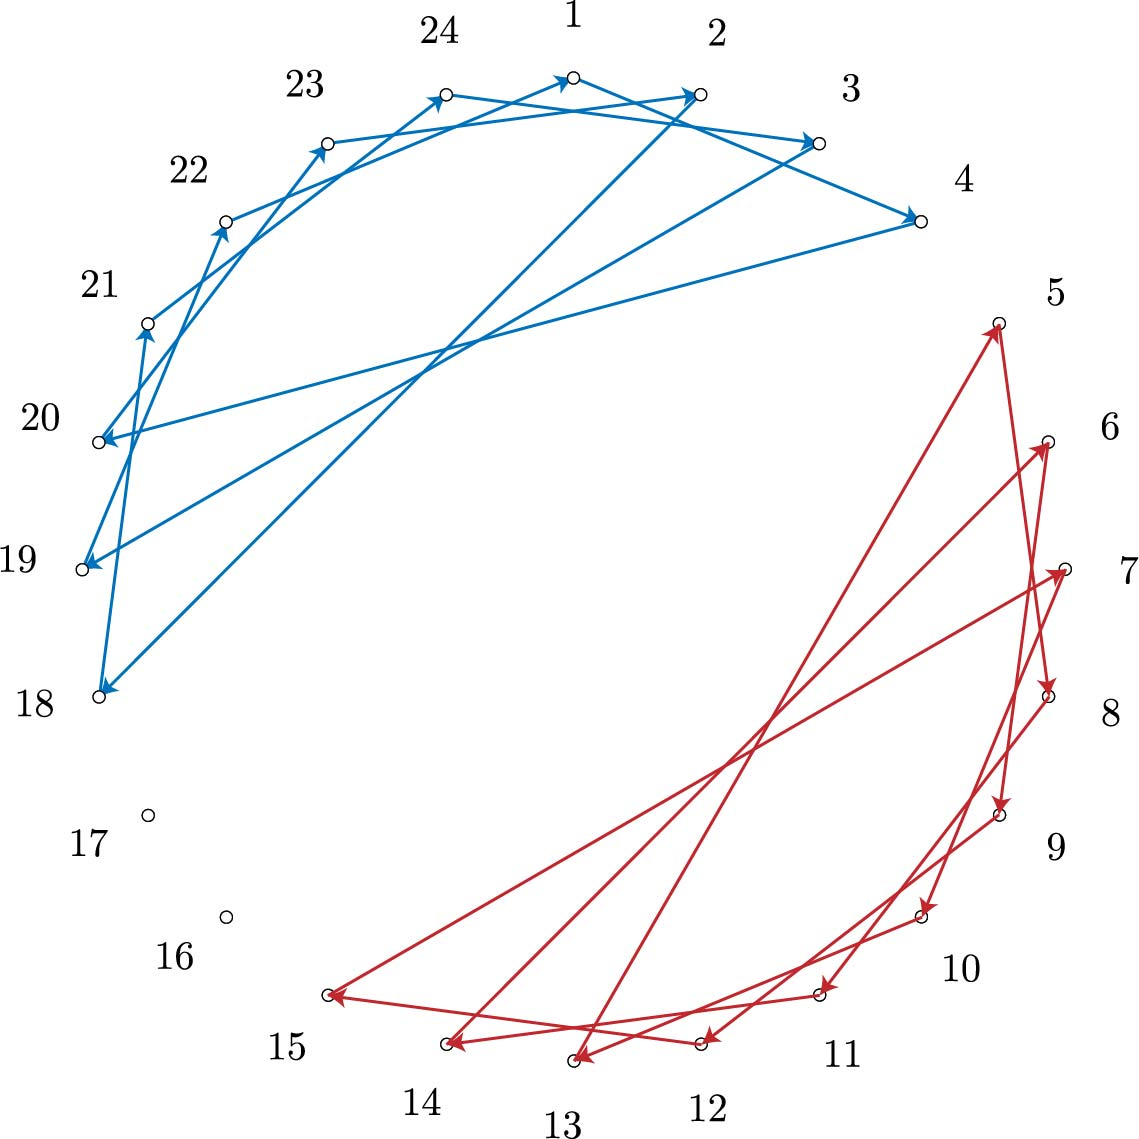
\includegraphics[scale=0.15]{circ_24_3_16_16_6.jpg}
		\caption{Nontrivial cycles for a permutation in
		$T_{24,3,16}(16,6)$. }
	\end{figure}


\end{frame}

%------------------------------------------------

\begin{frame}
\frametitle{Cycle Notation}
	\begin{Def}
		We define
		\begin{itemize}
			\item $r_i$ to be the number of $q_1$ steps in cycle
			$C_i$;
			\item $s_i$ to be the number of $q_2$ steps in cycle
			$C_i$;
			\item $l_i$ to be the weight of cycle $C_i$, given 
			by
			\bee
				l_i = \fracc{r_iq_1 + s_iq_2}{p}. 
			\eee
		\end{itemize}
	\end{Def}


\end{frame}

%------------------------------------------------

\begin{frame}
\frametitle{Cycle Notation}

	\begin{itemize}
		\item We represent each cycle $C_i$ by a 
		\textbf{starting point} $x_i$
		and a word $w_i$ (an ($r_i + s_i$)-tuple)
		specifying the \textbf{cycle steps} 
		from the starting point
		which define the cycle. 
		\item We write $C_i = (x_i;w_i)$. 
	\end{itemize}
	
	\begin{Ex}
		Consider the blue cycle in the figure. It is
		\bee
			C_1 = \text{(20 23 2 18 21 24 3 19 22 1 4)}. 
		\eee
		We write
		\bee
			C_1 &= (20; 
			q_1,q_1,q_2,q_1,q_1,q_1,q_2,q_1,q_1,q_1,q_2)\\
			&= (20; 3,3,16,3,3,3,16,3,3,3,16). 
		\eee
	\end{Ex}


\end{frame}

%------------------------------------------------

\begin{frame}
\frametitle{Cycle Example}

	\begin{figure}
		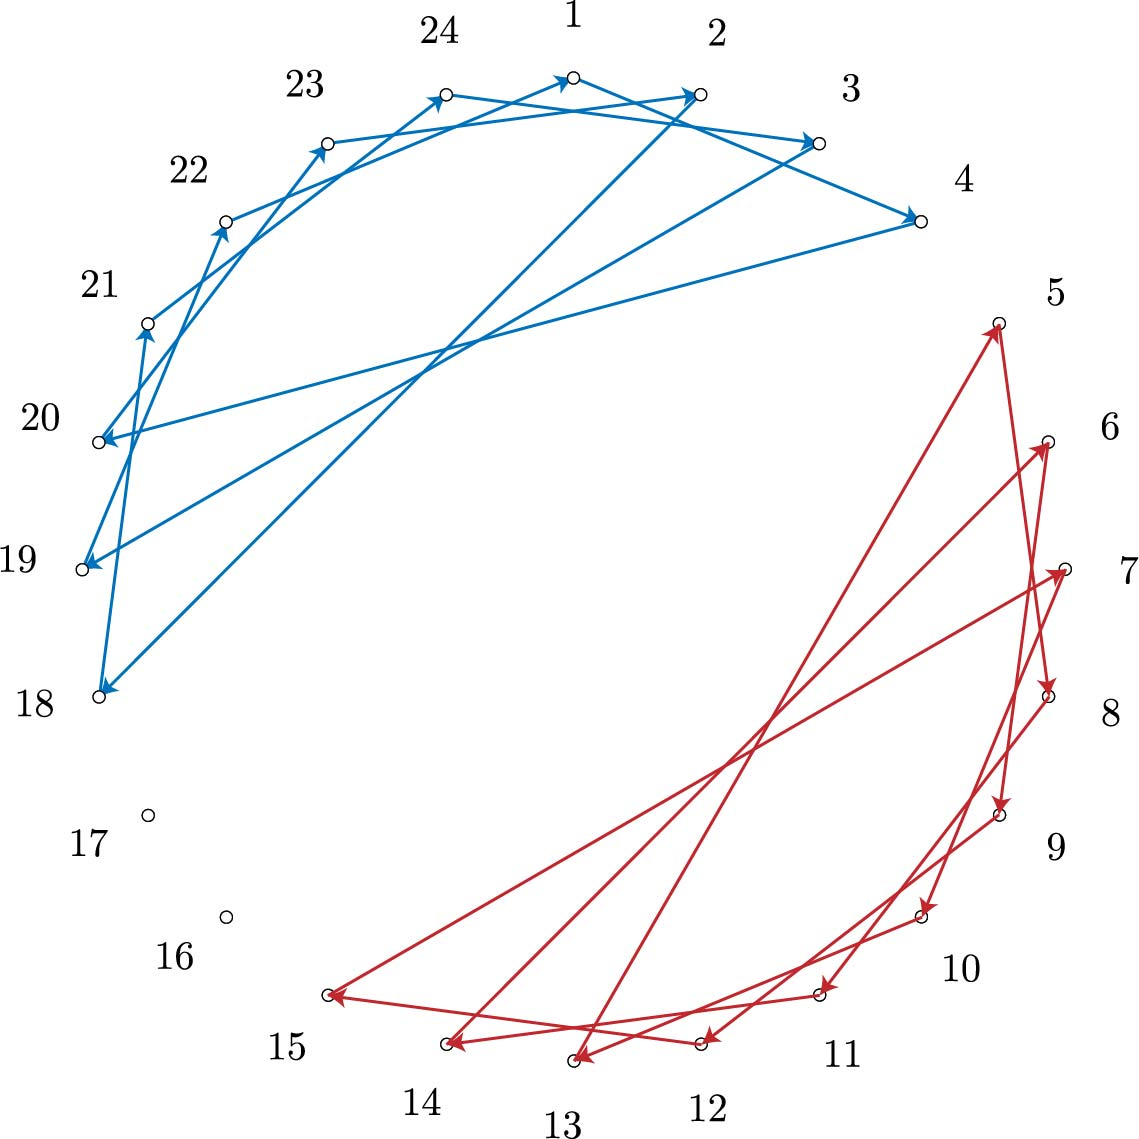
\includegraphics[scale=0.1]{circ_24_3_16_16_6.jpg}
		\caption{Nontrivial cycles for a permutation in
		$T_{24,3,16}(16,6)$. }
	\end{figure}
	\bee
		C_1 &= \text{(20 23 2 18 21 24 3 19 22 1 4)} \\
		&= (20; 3,3,16,3,3,3,16,3,3,3,16). 
	\eee

\end{frame}

%------------------------------------------------

\begin{frame}
\frametitle{Permutation/Cycle Image Notation}

	\begin{Def}
		We write
		$\sigma^t(i)$
		to denote the $t$-th image of 
		$i \in \Set{1,2,\hdots, p}$ under
		the permutation $\sigma$. 
		
		Similarly, we write
			$C_i^{\hspace{0.5mm}t}(i)$
		to denote the $t$-th image of $i$
		under the cycle $C_i$. 
	\end{Def}

\end{frame}

%------------------------------------------------

\begin{frame}
\frametitle{Two Lemmas}

	\begin{lem}
		If $T_{p,q_1,q_2}(r,s)$ is nonempty, 
		and $C_i$ is a cycle in $\sigma \in T_{p,q_1,q_2}(r,s)$
		then $p \mid (r_iq_1 + s_iq_2)$. 
		and $p \mid (rq_1 + sq_2)$. 
	\end{lem}
	
	\begin{lem}
		If $T_{p,q_1,q_2}(r,s)$ is nonempty, 
		then $\gcd(r_i,s_i,l_i) = 1$
		for all $1 \leq i \leq k$, for all
		$\sigma \in T_{p,q_1,q_2}(r,s)$. 
	\end{lem}
	
	\begin{itemize}
		\item We state these without proof for brevity. 
		\item They will be used later on. 
	\end{itemize}

\end{frame}

%------------------------------------------------

\begin{frame}
\frametitle{Definition of $m$-ordered sequence}
	\begin{itemize}
		\item Recall we are considering everything $\mod p$, 
	since all our permutations live in $S_p$. 
		\item We can consider our permutations
		as acting on elements
		of the set $\Set{1,2,\hdots, p}$. 
	\end{itemize}
	

\end{frame}

%------------------------------------------------

\begin{frame}
\frametitle{Definition of $m$-ordered sequence}
	\begin{Def}
	Let $x_1,x_2,\hdots, x_n \in \Set{1,2,\hdots, p}$, 
	and let $m \in \n$
	such that $1 \leq m \leq p - 1$. We say the 
	sequence $(x_1,x_2,\hdots, x_n)$ is $m$-ordered
	on $\Set{1,2,\hdots, p}$ if 
	\begin{enumerate}
		\item $3 \leq n \leq \fracc{\mathrm{lcm}(p,m)}{m}$;
		\item $x_i \equiv x_j (\mod \gcd(p,m))$ for all
		$i,j$;
		\item In the clockwise traversal of 
		$\Set{1,2,\hdots, p}$ by
		$m$-steps, starting with $x_1$, we hit $x_i$ before
		$x_j$ if and only if $i < j$. 
	\end{enumerate}
	\end{Def}	

\end{frame}

%------------------------------------------------

\begin{frame}
\frametitle{Definition of $m$-ordered sequence}
	This is an opaque definition. Let's break it down. 
	\begin{block}{Condition 1}
		\bee
			3 \leq n \leq \fracc{\mathrm{lcm}(p,m)}{m}
		\eee
	\end{block}
	\begin{itemize}
		\item We require that $n \geq 3$ since our 
		definition is not 
		meaningful with less than $3$ points. 
		\item Otherwise, any two point sequence which satisfies 
		condition \#2 would be $m$-ordered. 
	\end{itemize}
	

\end{frame}

%------------------------------------------------

\begin{frame}
\frametitle{Definition of $m$-ordered sequence}
	\begin{block}{Condition 1}
		\bee
			3 \leq n \leq \fracc{\mathrm{lcm}(p,m)}{m}
		\eee
	\end{block}
	\begin{itemize}
		\item Note that $\mathrm{lcm}(p,m)$ is the 
		maximum ``distance'' you can move around the 
		circle when traversing by $m$-steps before
		coming back to the same point. 
	\end{itemize}
	

\end{frame}

%------------------------------------------------

\begin{frame}
\frametitle{Definition of $m$-ordered sequence}
	\begin{itemize}
		\item Note that $\mathrm{lcm}(p,m)$ is the 
		maximum ``distance'' you can move around the 
		circle when traversing by $m$-steps before
		coming back to the same point. 
		\item If $p$ and $m$ are coprime, then
		$\mathrm{lcm}(p,m) = pm$. 
	\end{itemize}
	\begin{figure}
		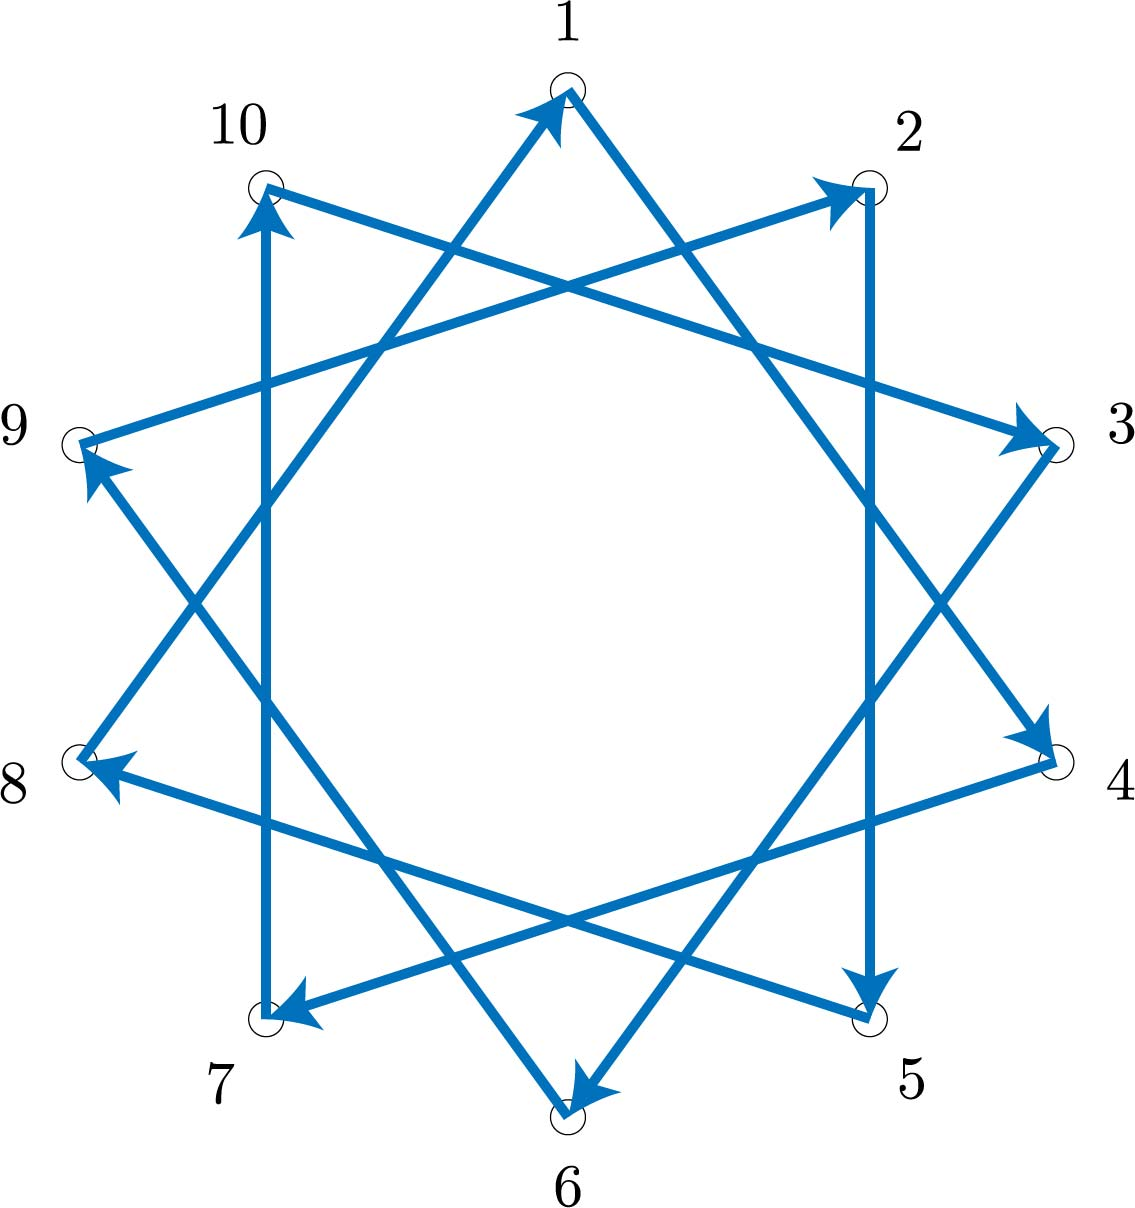
\includegraphics[scale=0.08]{circ_10_3.jpg}
		\caption{Note $10$ and $3$ are coprime, so
		we cover $\lcm(10,3) = 30$ points, or three
		full rotations before coming back to the starting point. }
	\end{figure}
	
\end{frame}

%------------------------------------------------

\begin{frame}
\frametitle{Definition of $m$-ordered sequence}
	\begin{itemize}
		\item Note that $\mathrm{lcm}(p,m)$ is the 
		maximum ``distance'' you can move around the 
		circle when traversing by $m$-steps before
		coming back to the same point. 
	\end{itemize}
	\begin{figure}
		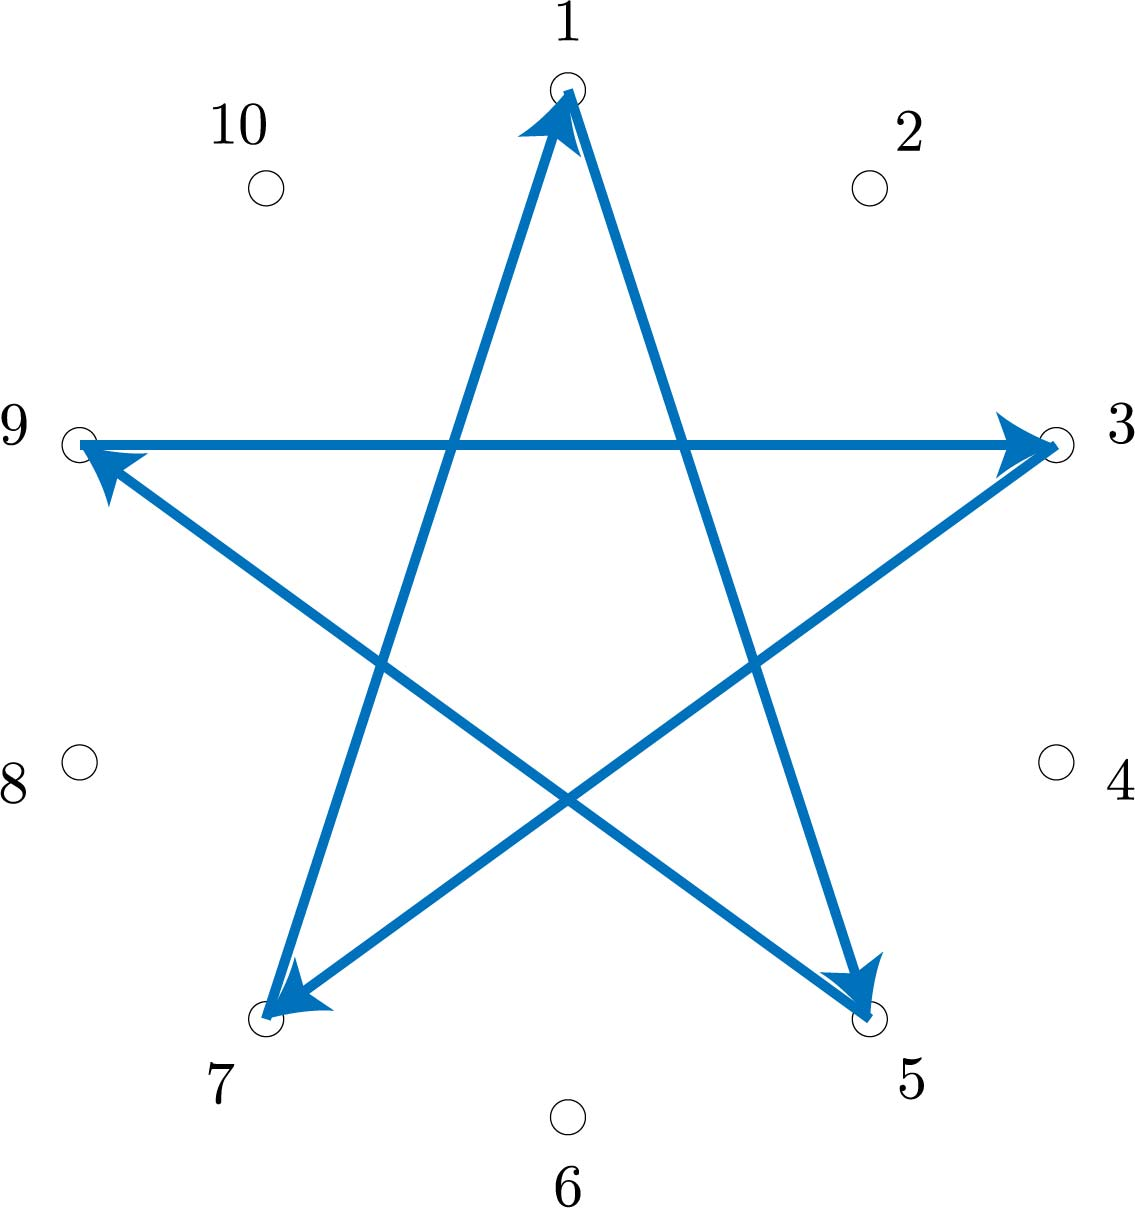
\includegraphics[scale=0.08]{circ_10_4.jpg}
		\caption{When $p = 10$, and $m = 4$, we 
		pass $\lcm(10,4) = 20$ points 
		before coming back to the starting point. }
	\end{figure}
	
\end{frame}

%------------------------------------------------

\begin{frame}
\frametitle{Definition of $m$-ordered sequence}
	\begin{itemize}
		\item If we want to know the maximum number
		of $m$-steps we can take before coming back
		to the starting point (i.e. the longest 
		possible sequence which makes sense), 
		we just divide the number of points we pass
		$\lcm(p,m)$ by the size of each step $m$. 
	\end{itemize}
	\begin{figure}
		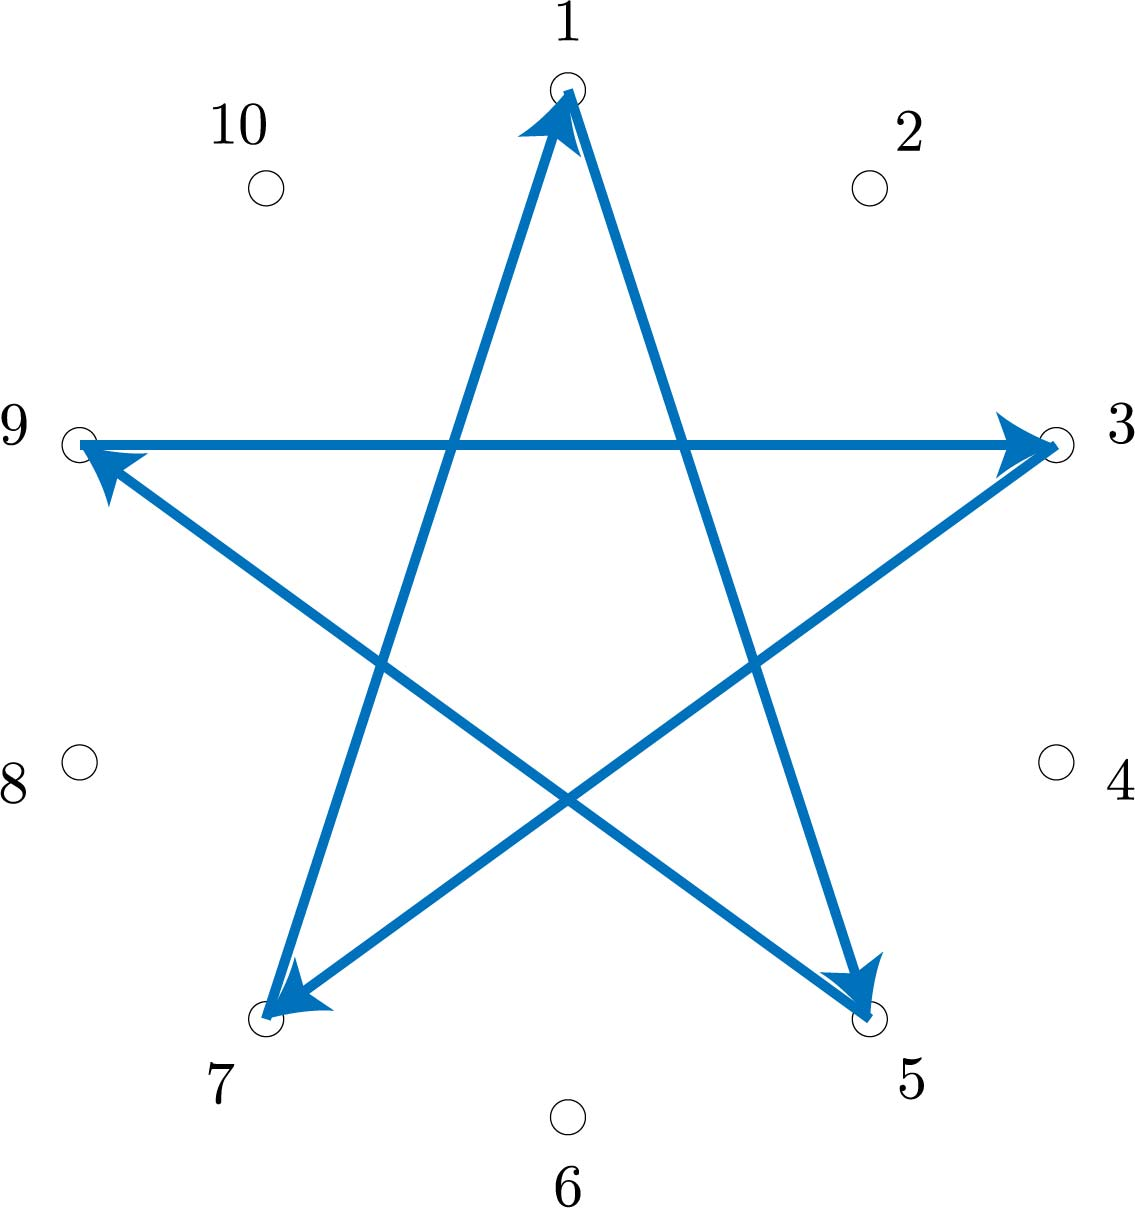
\includegraphics[scale=0.08]{circ_10_4.jpg}
		\caption{Note $\lcm(10,4) = 20$. So we pass 
		$20$ points taking size $4$ steps, so 
		we can take at most $20/4 = 5$ steps before
		coming back to the same spot. }
	\end{figure}
	
\end{frame}

%------------------------------------------------

\begin{frame}
\frametitle{Definition of $m$-ordered sequence}
	Hence:
	\begin{block}{Condition 1}
		\bee
			3 \leq n \leq \fracc{\mathrm{lcm}(p,m)}{m}
		\eee
	\end{block}
	
\end{frame}

%------------------------------------------------

\begin{frame}
\frametitle{Definition of $m$-ordered sequence}
	\begin{block}{Condition 2}
	\bee
			x_i \equiv x_j \mod \gcd(p,m) \text{ for all }
			i,j
	\eee
	\end{block}
	
	\begin{itemize}
		\item Condition 2 tells us nothing if $\gcd(p,m) = 1$. 
		\item When the $\gcd$ is greater than $1$, 
		Condition 2 simply tells us that all
		elements in the sequence are in the same equivalence
		class $\mod p$ generated by $m$-steps. 
	\end{itemize}
	
\end{frame}

%------------------------------------------------

\begin{frame}
\frametitle{Definition of $m$-ordered sequence}

	\begin{figure}
		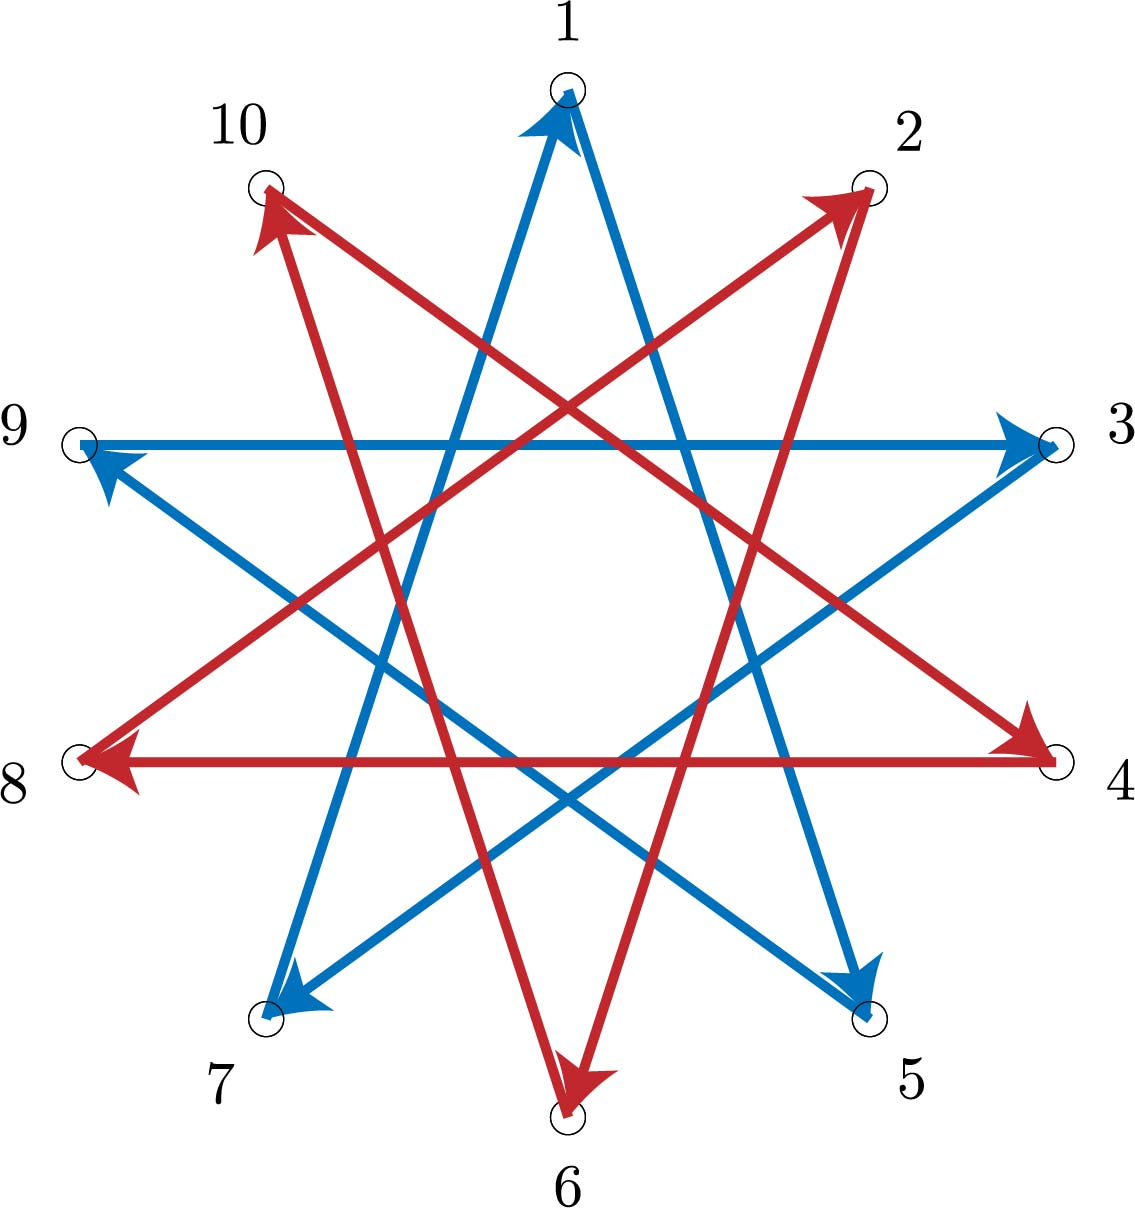
\includegraphics[scale=0.1]{circ_10_4_equiv.jpg}
		\caption{The two equivalence classes $\mod 10$
		generated by taking $4$-steps in 
		$\Set{1,2,\hdots, 10}$. }
	\end{figure}
	
\end{frame}

%------------------------------------------------

\begin{frame}
\frametitle{Definition of $m$-ordered sequence}

	\begin{block}{Condition 3}
		In the clockwise traversal of 
		$\Set{1,2,\hdots, p}$ by
		$m$-steps, starting with $x_1$, we hit $x_i$ before
		$x_j$ if and only if $i < j$. 
	\end{block}
	\begin{itemize}
		\item We give some intuition for this notion
		with a few examples. 
	\end{itemize}
	
\end{frame}

%------------------------------------------------

\begin{frame}
\frametitle{Definition of $m$-ordered sequence}

	Consider sequences of elements in $\Set{1,2,\hdots, 10}$. 

	\begin{figure}
		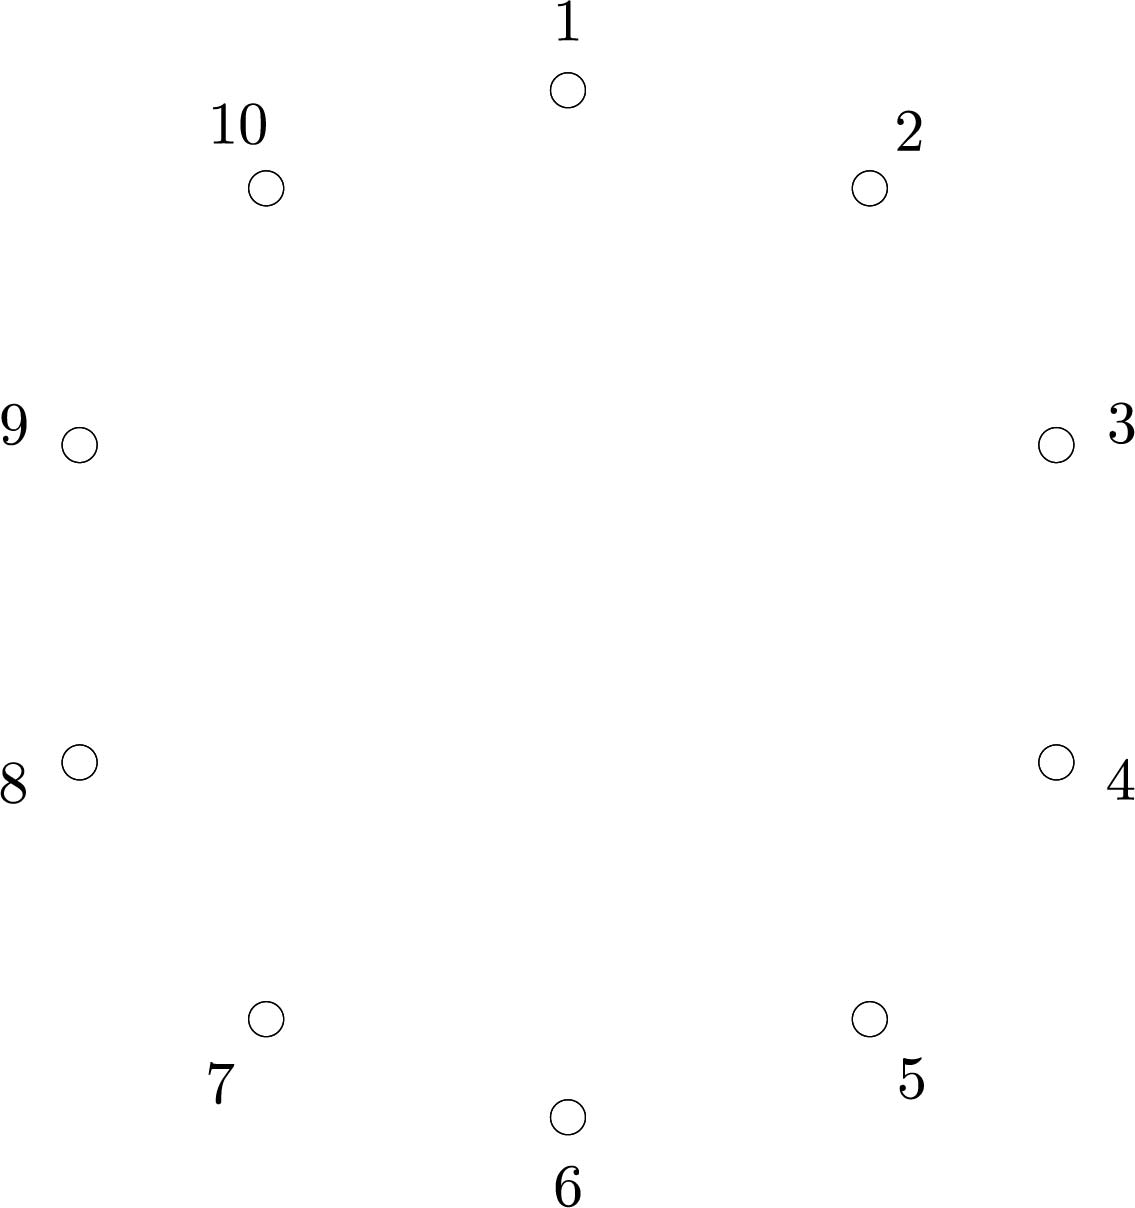
\includegraphics[scale=0.1]{circ_10.jpg}
	\end{figure}
	
	\begin{question}
		Is $(1,2,3,4)$ $1$-ordered?
	\end{question}
	
\end{frame}

%------------------------------------------------

\begin{frame}
\frametitle{Definition of $m$-ordered sequence}

	Consider sequences of elements in $\Set{1,2,\hdots, 10}$. 

	\begin{figure}
		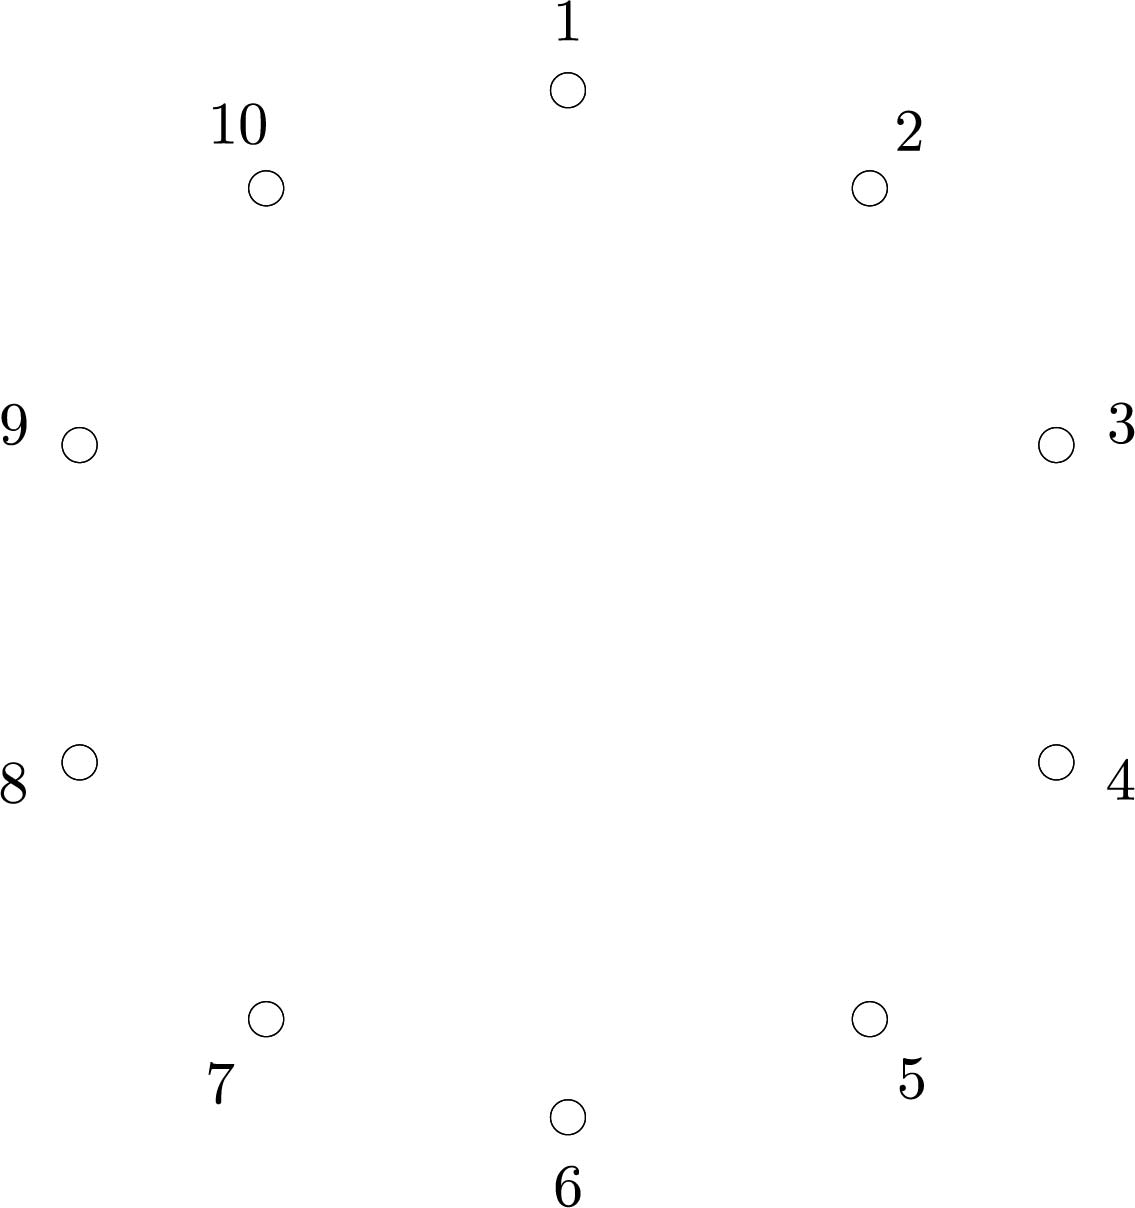
\includegraphics[scale=0.1]{circ_10.jpg}
	\end{figure}
	
	\begin{question}
		Is $(1,2,3,5)$ $1$-ordered?
	\end{question}
	
\end{frame}

%------------------------------------------------

\begin{frame}
\frametitle{Definition of $m$-ordered sequence}

	Consider sequences of elements in $\Set{1,2,\hdots, 10}$. 

	\begin{figure}
		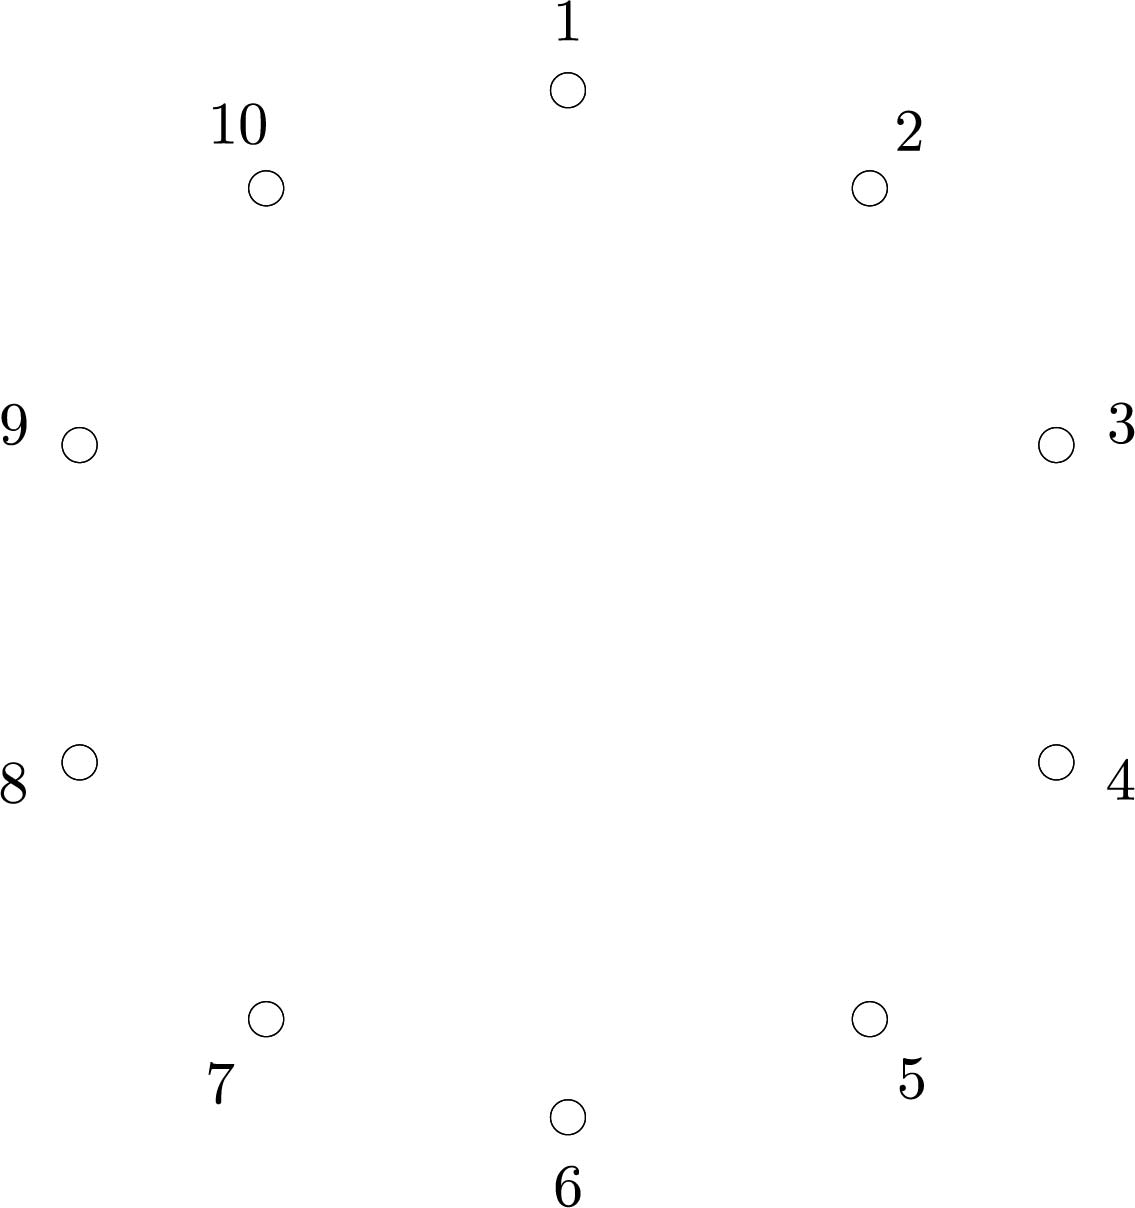
\includegraphics[scale=0.1]{circ_10.jpg}
	\end{figure}
	
	\begin{question}
		Is $(1,2,4,3)$ $1$-ordered?
	\end{question}
	
\end{frame}

%------------------------------------------------

\begin{frame}
\frametitle{Definition of $m$-ordered sequence}

	Consider sequences of elements in $\Set{1,2,\hdots, 32}$. 

	\begin{figure}
		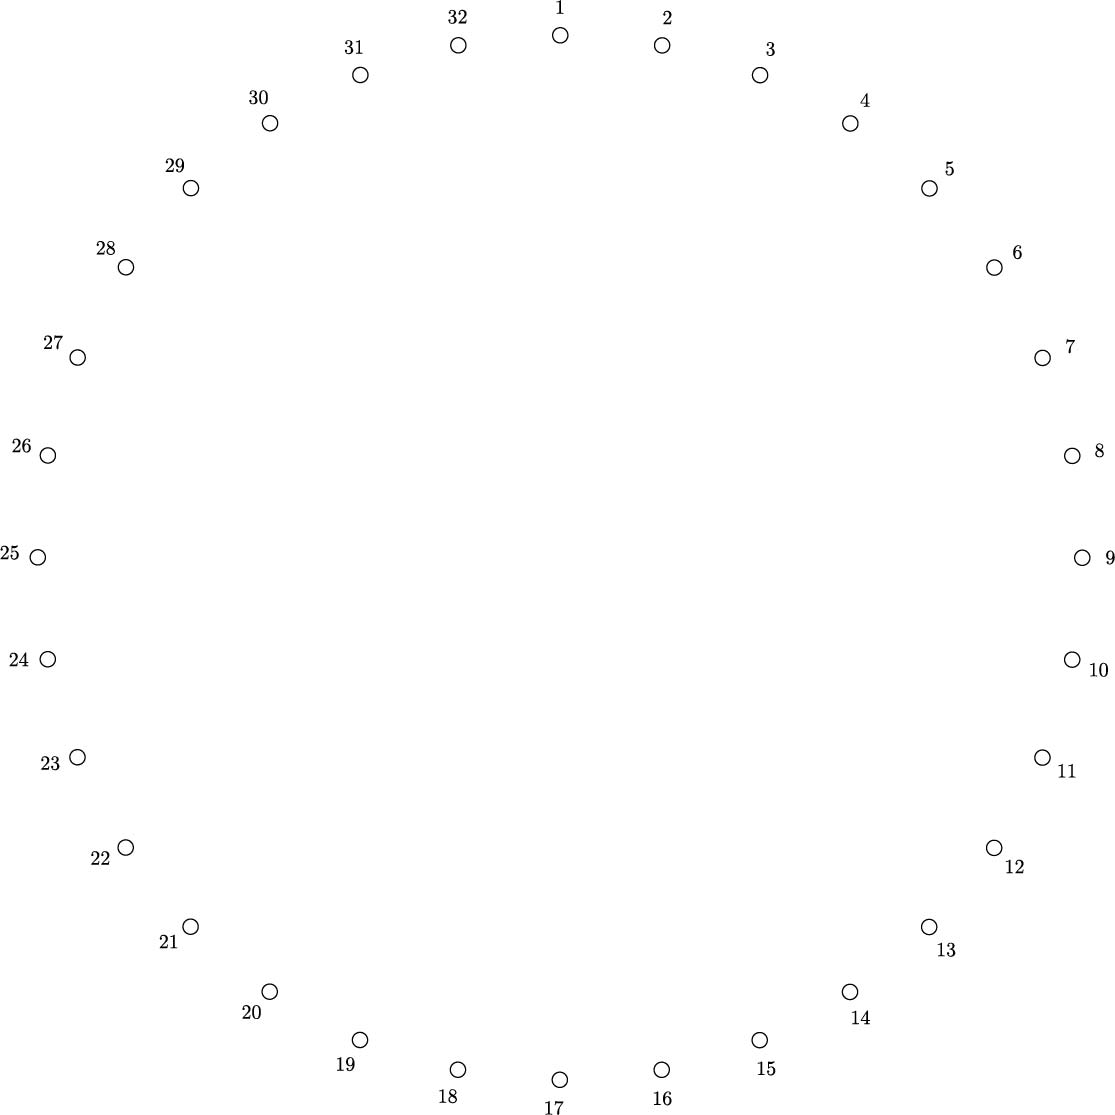
\includegraphics[scale=0.1]{circ_32_3_12_12_5.jpg}
	\end{figure}
	
	\begin{question}
		Is $(3,8,13)$ $5$-ordered?
	\end{question}
	
\end{frame}

%------------------------------------------------

\begin{frame}
\frametitle{Definition of $m$-ordered sequence}

	Consider sequences of elements in $\Set{1,2,\hdots, 32}$. 

	\begin{figure}
		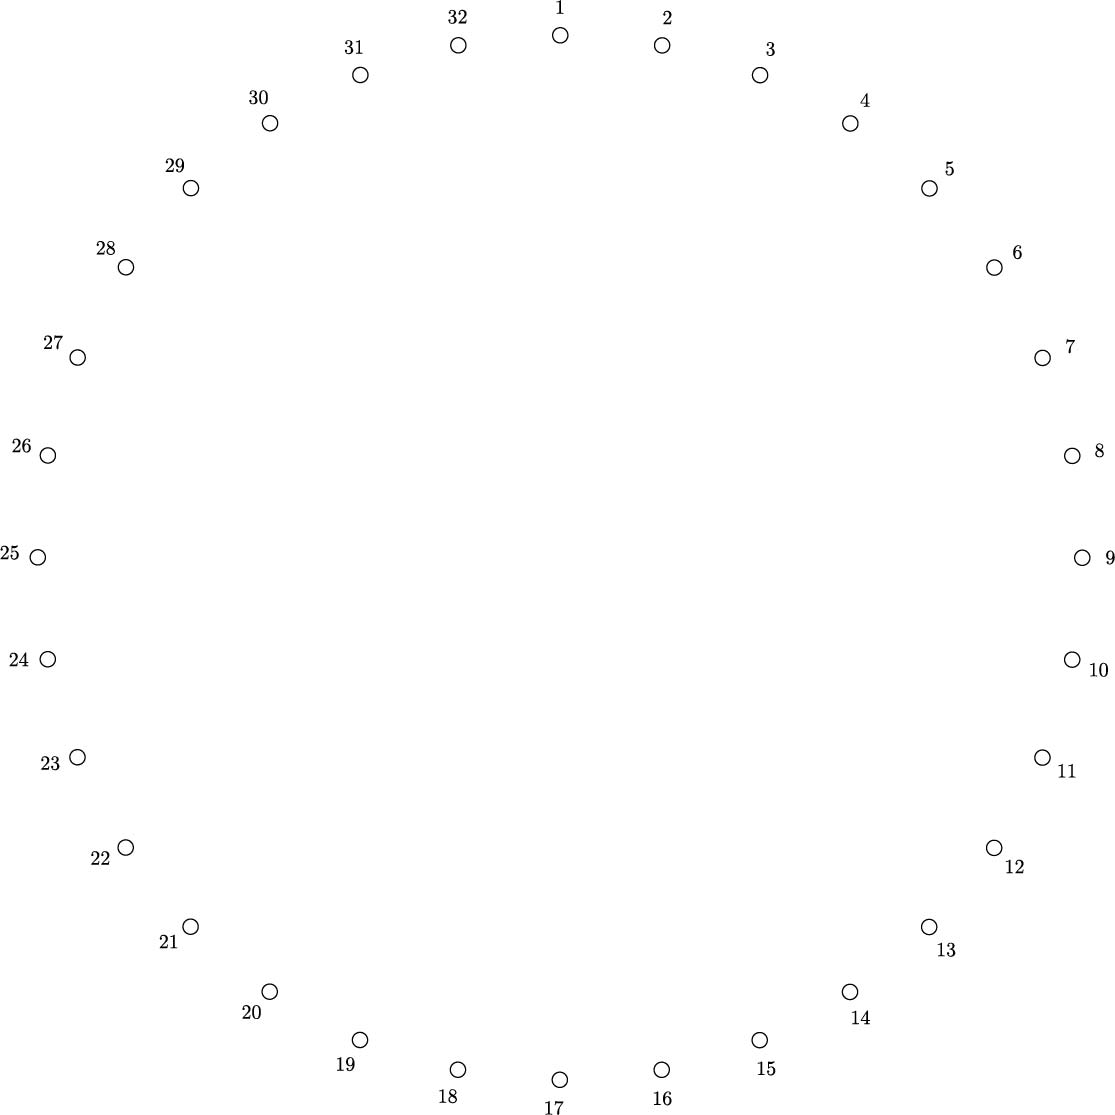
\includegraphics[scale=0.1]{circ_32_3_12_12_5.jpg}
	\end{figure}
	
	\begin{question}
		Is $(3,13,18)$ $5$-ordered?
	\end{question}
	
\end{frame}

%------------------------------------------------

\begin{frame}
\frametitle{Definition of $m$-ordered sequence}

	Consider sequences of elements in $\Set{1,2,\hdots, 10}$. 

	\begin{figure}
		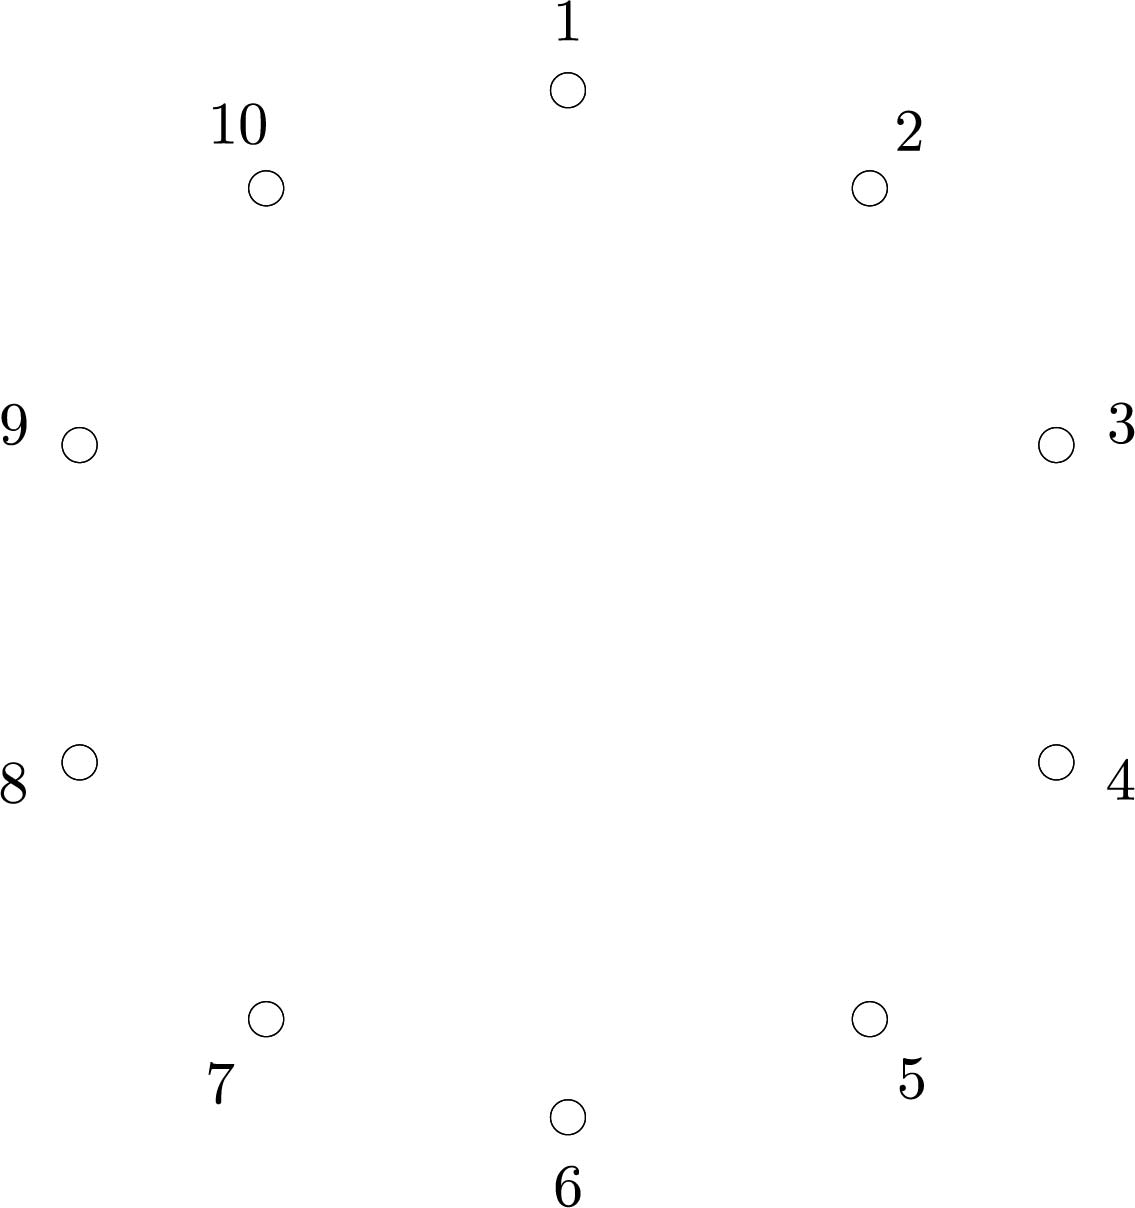
\includegraphics[scale=0.1]{circ_10.jpg}
	\end{figure}
	
	\begin{question}
		Is $(1,4,2,5)$ $3$-ordered?
	\end{question}
	
\end{frame}

%------------------------------------------------

\begin{frame}
\frametitle{Definition of $m$-ordered sequence}

	Consider sequences of elements in $\Set{1,2,\hdots, 10}$. 

	\begin{figure}
		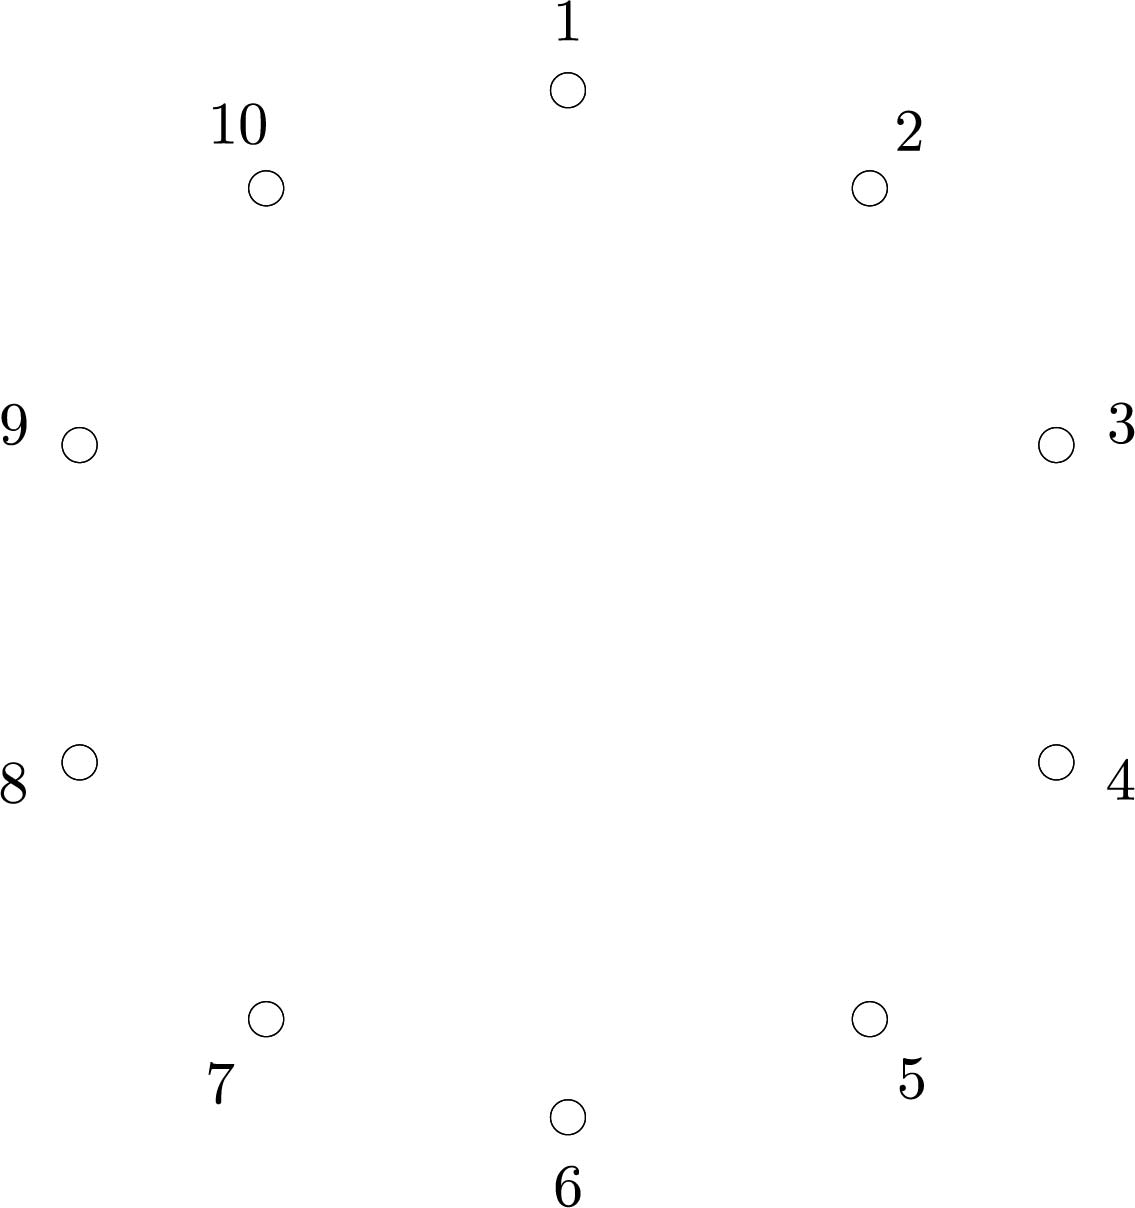
\includegraphics[scale=0.1]{circ_10.jpg}
	\end{figure}
	
	\begin{question}
		Is $(2,5,6,3)$ $3$-ordered?
	\end{question}
	
\end{frame}

%------------------------------------------------

\begin{frame}
\frametitle{Definition of $m$-ordered sequence}

	Consider sequences of elements in $\Set{1,2,\hdots, 10}$. 

	\begin{figure}
		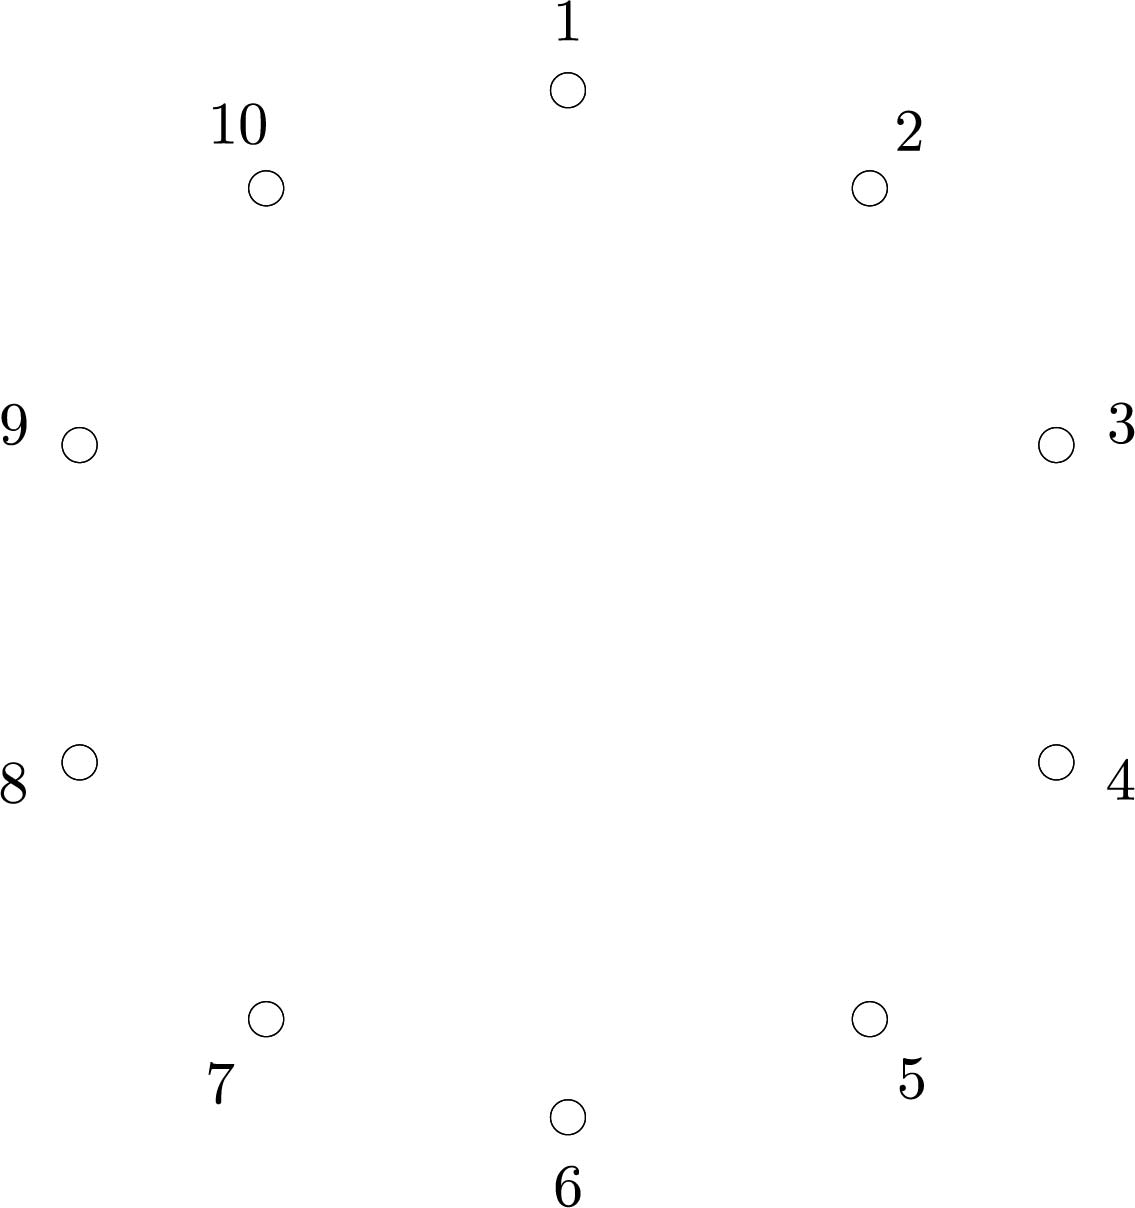
\includegraphics[scale=0.1]{circ_10.jpg}
	\end{figure}
	
	\begin{question}
		Is $(1,5,3)$ $4$-ordered? Is it $2$-ordered?
	\end{question}
	
\end{frame}

%------------------------------------------------

\begin{frame}
\frametitle{Definition of $m$-ordered sequence}
	\begin{Def}
	Let $x_1,x_2,\hdots, x_n \in \Set{1,2,\hdots, p}$, 
	and let $m \in \n$
	such that $1 \leq m \leq p - 1$. We say the 
	sequence $(x_1,x_2,\hdots, x_n)$ is $m$-ordered
	on $\Set{1,2,\hdots, p}$ if 
	\begin{enumerate}
		\item $3 \leq n \leq \fracc{\mathrm{lcm}(p,m)}{m}$;
		\item $x_i \equiv x_j (\mod \gcd(p,m))$ for all
		$i,j$;
		\item In the clockwise traversal of 
		$\Set{1,2,\hdots, p}$ by
		$m$-steps, starting with $x_1$, we hit $x_i$ before
		$x_j$ if and only if $i < j$. 
	\end{enumerate}
	\end{Def}	

\end{frame}

%------------------------------------------------

\begin{frame}
\frametitle{Proving Identical Cycle Structure}
	\begin{lem}
		If $\sigma \in T_{p,q_1,q_2}(r,s)$, 
		and 
		$\gcd(p,q_1,q_2) = 1$, we must have
		$r_1 = r_2 = \cdots = r_k$ and 
		$s_1 = s_2 = \cdots = s_k$. 
	\end{lem}
	
	\begin{itemize}
		\item ``All cycles in a permutation from 
		$T_{p,q_1,q_2}(r,s)$ have the same number of 
		$q_1$-steps and the same number of $q_2$-steps.''
	\end{itemize}

\end{frame}

%------------------------------------------------

\begin{frame}
\frametitle{Proving Identical Cycle Structure}
	
	\begin{itemize}
		\item Let $C_k,C_l$ be two distinct, nontrivial cycles in 
		$\sigma \in T_{p,q_1,q_2}(r,s)$. 
		\item We write $C_k = (x_k;w_k)$ using
		our \textbf{starting-point/step-vector} notation. 
		\item And we group all $q_1$-steps together which
		precede each $q_2$-step, so we have
		\bee
			w_k = (q_1^{\rho_1},q_2,\hdots, q_1^{\rho_{s_k}}, q_2)
		\eee
		where $\sum \rho_i = r_k$, the number of $q_1$ steps
		in the cycle. 
	\end{itemize}
	

\end{frame}

%------------------------------------------------

\begin{frame}
\frametitle{Proving Identical Cycle Structure}
	
	\begin{block}{Grouping $q_1$-steps example}
		Recall our example cycle from
		a permutation in $T_{24,3,16}(16,6)$:
		\bee
			C_1 = \text{(20 23 2 18 21 24 3 19 22 1 4)}. 
		\eee
		We write
		\bee
			C_1 &= (20; 
			q_1,q_1,q_2,q_1,q_1,q_1,q_2,q_1,q_1,q_1,q_2)\\
			&= (20; 3,3,16,3,3,3,16,3,3,3,16) \\
			&= (20;3^2,16,3^3,16,3^3,16) \\
			&= (x_i; q_1^{\rho_1},q_2,q_1^{\rho_2}
				q_2, q_1^{\rho_3},q_2). 
		\eee
	\end{block}
	

\end{frame}

%------------------------------------------------

\begin{frame}
\frametitle{Proving Identical Cycle Structure}

	\begin{figure}
		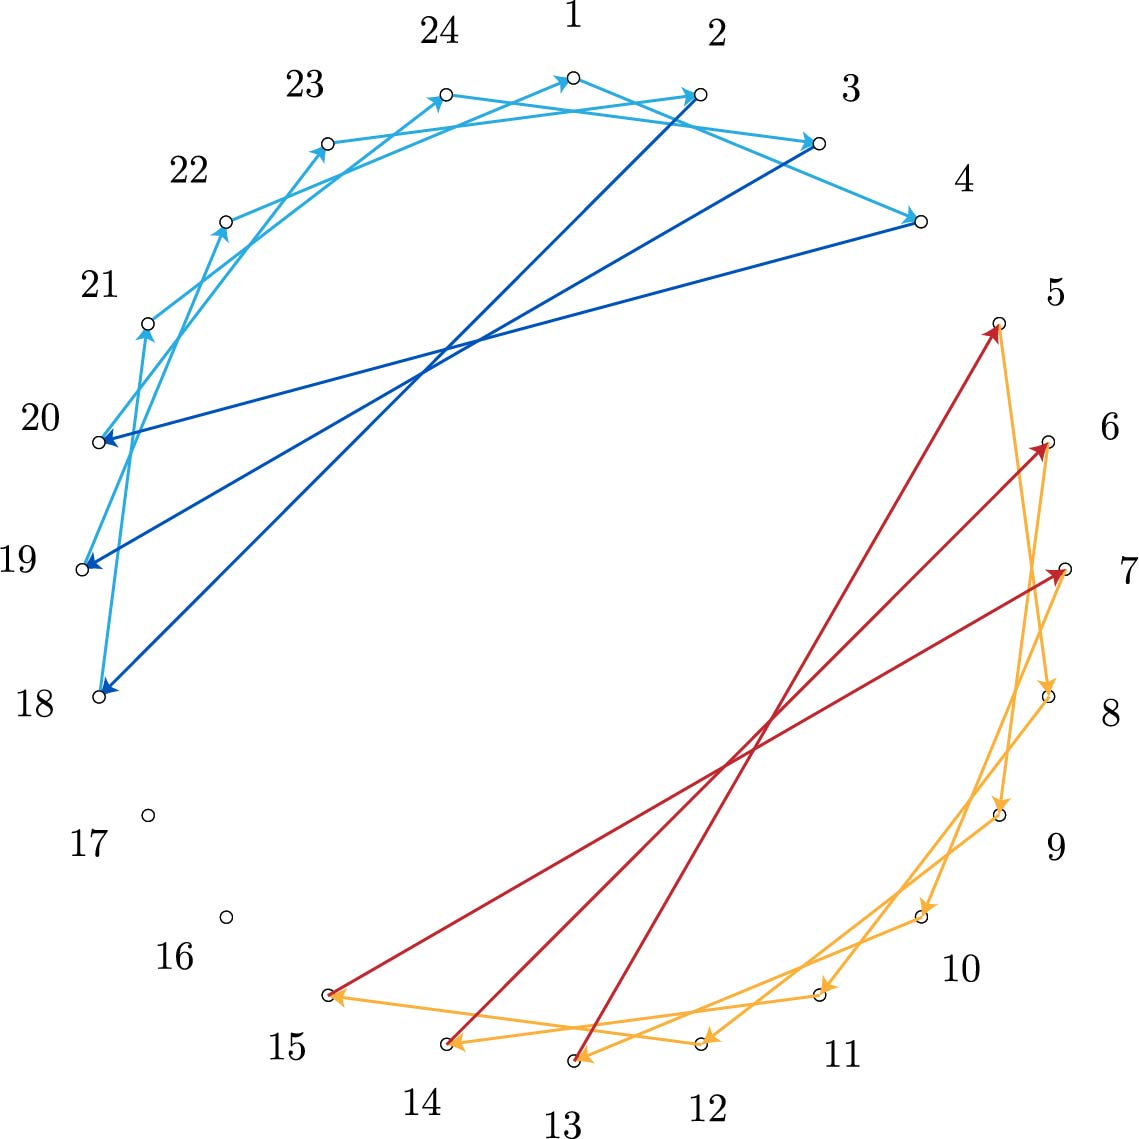
\includegraphics[scale=0.1]{circ_24_3_16_16_6_colored.jpg}
		\caption{$q_2$-steps from $C_1$ are in dark blue, and 
		$q_2$-steps from $C_2$ are in red. }
	\end{figure}
	\vspace{-5mm}
	\begin{block}{Identical Number of $q_2$-steps}
		We proceed to show $s_k = s_l$, i.e.
		the number of $q_2$-steps in $C_k$ is the
		same as the number of $q_2$-steps in $C_l$. 
	\end{block}
	

\end{frame}

%------------------------------------------------

\begin{frame}
\frametitle{Proving Identical Cycle Structure}

	\begin{itemize}
		\item We first argue that $s_l \geq s_k$. 
		\item If $s_k = 0$, there is nothing to prove, 
		so assume $s_k \geq 1$, i.e. we have at least
		one $q_2$-step in $C_k$. 
	\end{itemize}
	\begin{block}{Defining $e_i$ points and $d_i$ points}
		We enumerate the $q_2$-steps (we use the term
		$q_2$-step here to denote a point
		from which we jump $q_2$ points on the circle)
		as $\Set{e_i}$, and the images of the 
		$q_2$-steps as $\Set{d_i}$, where $1 \leq i \leq s_k$. 
	\end{block}
	

\end{frame}

%------------------------------------------------

\begin{frame}
\frametitle{Proving Identical Cycle Structure}

	\begin{figure}
		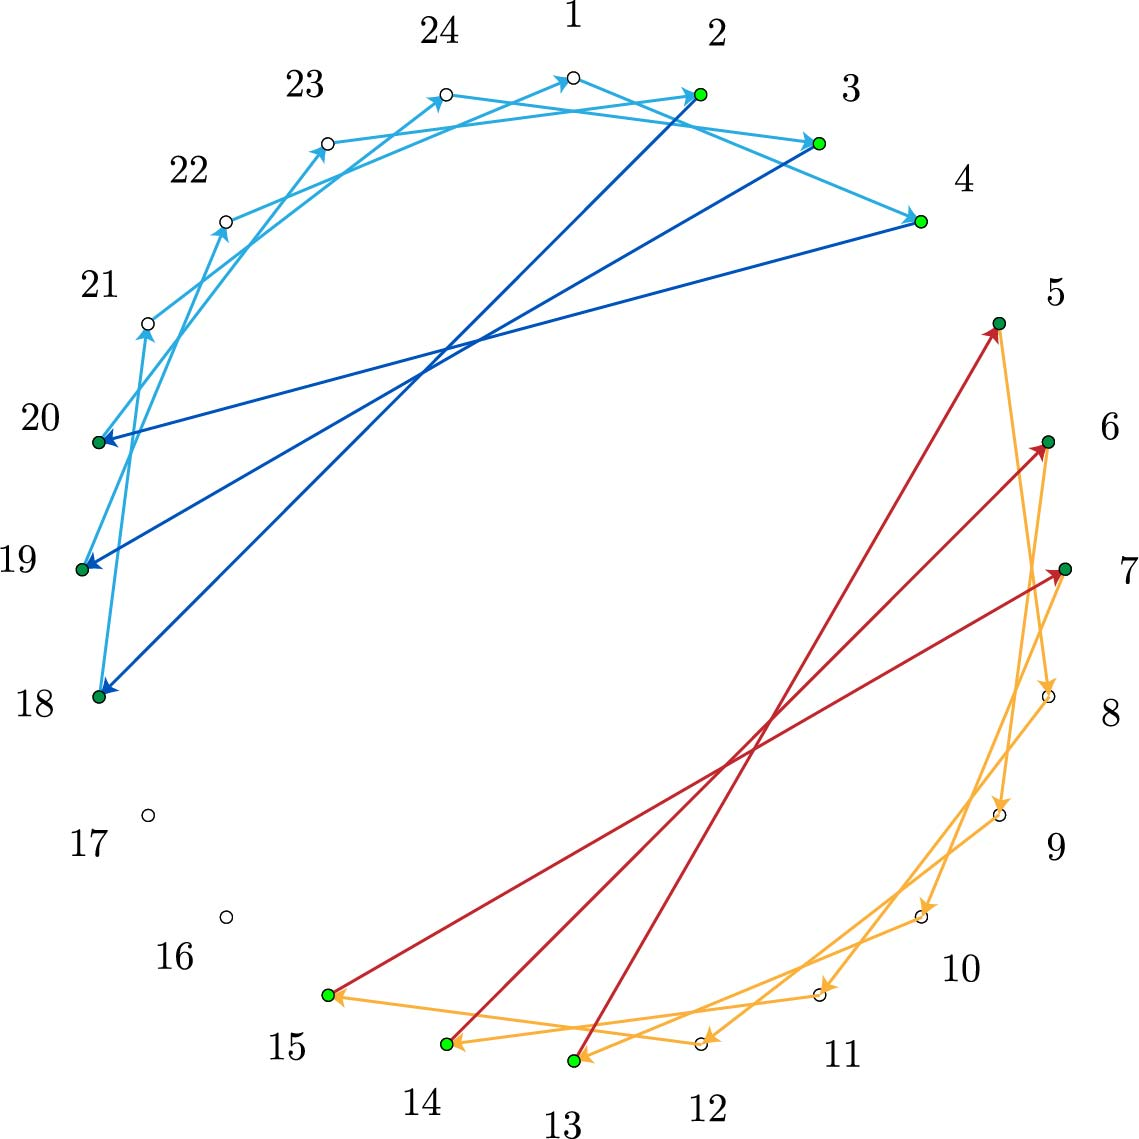
\includegraphics[scale=0.15]{circ_24_3_16_16_6_ed.jpg}
		\caption{The $\Set{e_i}$ points ($q_2$-steps)
		are light-green, and the $\Set{d_i}$ points (images of 
		$q_2$-steps) are in dark-green. }
	\end{figure}
	

\end{frame}

%------------------------------------------------

\begin{frame}
\frametitle{Proving Identical Cycle Structure}

	\begin{block}{Labeling the $e_i$ and $d_i$ points}
		\begin{itemize}
			\item Recall
			\bee
				C_k 
				&=
					\lpar 
						x_k; (q_1^{\rho_1},q_2,\hdots, 
						q_1^{\rho_{s_k}},q_2)
					\rpar. 
			\eee
			\item Set $d_1 = x_k$. 
			\item Set $e_1 = C_k^{\hspace{0.5mm}\rho_1}(x_k)$. 
			\item If $s_k > 1$, iteratively define
			\bee
				d_i &= C_k(e_{i - 1})\\
				e_i &= C_k^{\hspace{0.5mm}\rho_i}(d_i)
			\eee
			for $1 \leq i \leq s_k$. 
		\end{itemize}
	\end{block}
	

\end{frame}

%------------------------------------------------

\begin{frame}
\frametitle{Proving Identical Cycle Structure}

	\begin{Ex}
		Recall
		\bee
			C_1 &= \text{(20 23 2 18 21 24 3 19 22 1 4)} \\
			&= (20;3^2,16,3^3,16,3^3,16) \\
			&= (x_i; q_1^{\rho_1},q_2,q_1^{\rho_2}
			q_2, q_1^{\rho_3},q_2). 
		\eee
		So
		\bee
			d_1 &= 20; && e_1 = 2; \\
			d_2 &= 18; && e_2 = 3; \\
			d_3 &= 19; && e_3 = 4. 
		\eee
	\end{Ex}
	

\end{frame}

%------------------------------------------------

\begin{frame}
\frametitle{Proving Identical Cycle Structure}

	\begin{Claim}
		We assert that there exists a unique permutation
		$U \in S_{s_k}$ such that 
		\begin{enumerate}
			\item If $e_j = d_j$, then $U(j) = j$. 
			\item If $e_j \neq d_j$, then
			for any $x \in \Set{1,2,\hdots, p}$
			such that $(e_j,x,d_{U(j)})$ is $q_1$-ordered,
			$x \notin \Set{d_i}$. 
		\end{enumerate}
		
		
	\end{Claim}
	\begin{block}{Intuition}
		We assert that for each $q_2$-step
		($e$ point), we have a $d$ point
		which is ``hit'' first when we traverse
		$\Set{1,2,\hdots, p}$ by $q_1$-steps 
		starting from the $e$ point, and these
		are distinct for each distinct $e$ point. 
		If the $d$ point is also an $e$ point, 
		we let $U(j) = j$ and say that the $e$ 
		point itself is the first $d$ point we hit. 
	\end{block}
	

\end{frame}

%------------------------------------------------

\begin{frame}
\frametitle{Proving Identical Cycle Structure}

	\begin{figure}
		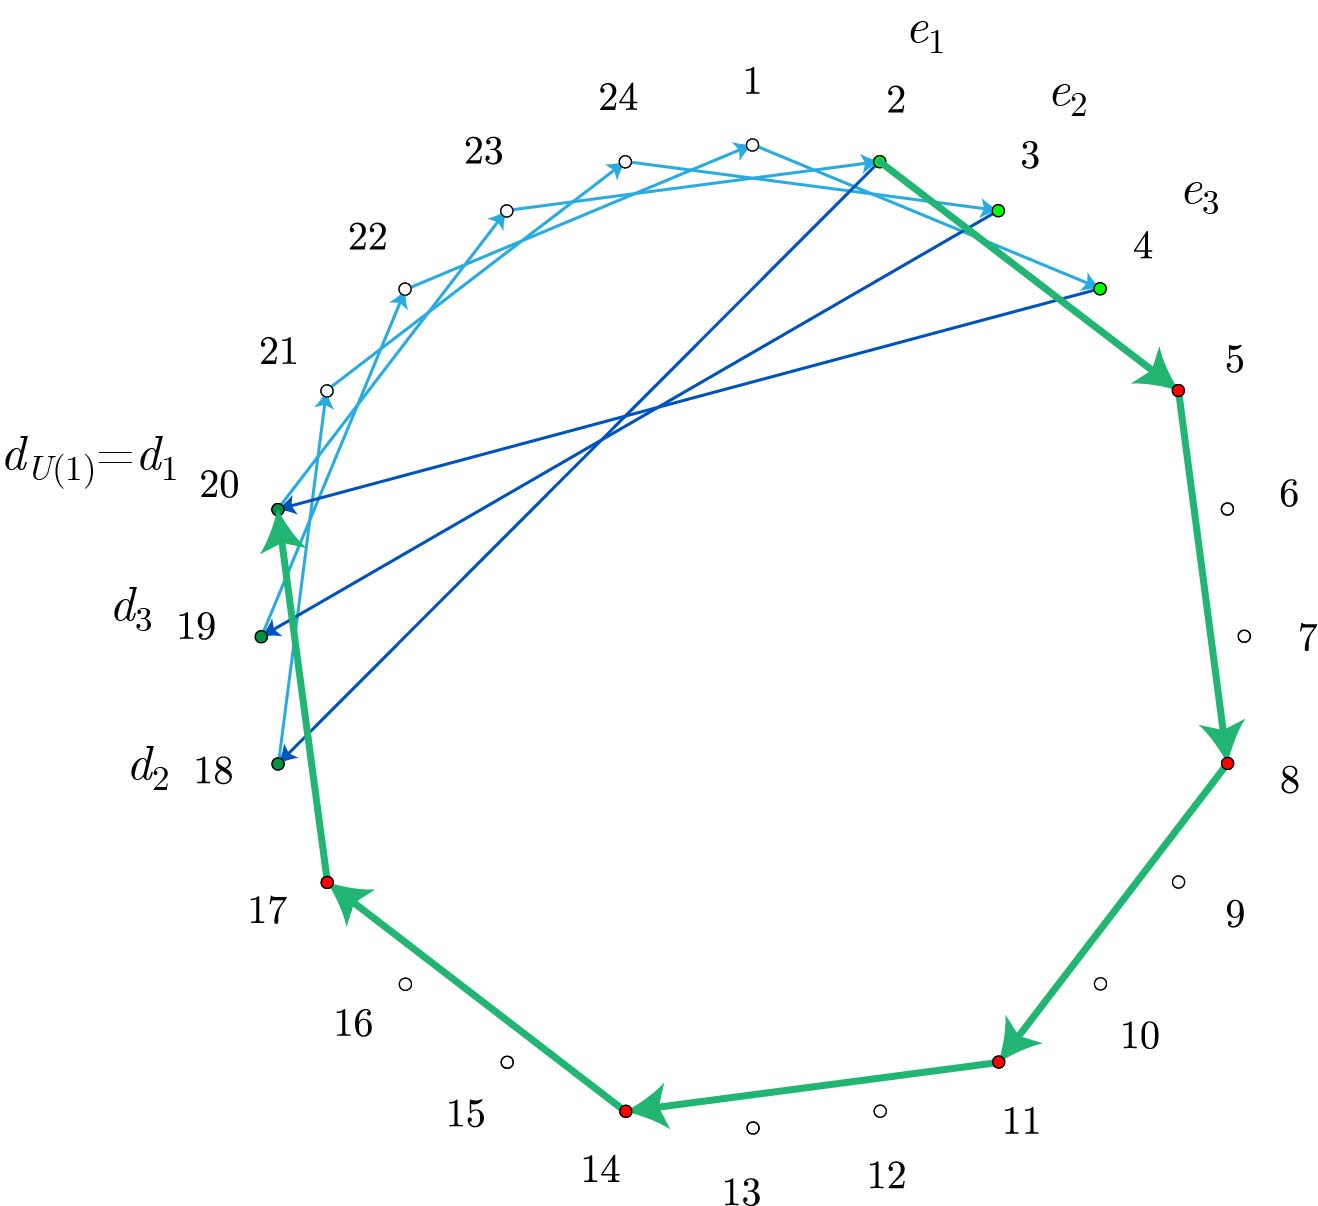
\includegraphics[scale=0.15]{circ_24_U.jpg}
		\caption{Finding $U(1)$ for cycle $C_1$ 
		in a permutation in $T_{24,3,16}(16,6)$. 
		The points in red are all $x \in \Set{1,2,
		\hdots, 24}$ for which $(e_1,x,d_1)$ is $q_1$-ordered. }
	\end{figure}

\end{frame}

%------------------------------------------------

\begin{frame}
\frametitle{Proving Identical Cycle Structure}

	\begin{question}
		When could the claim be false?
	\end{question}
	
	\begin{itemize}
		\item It could be false if when traversing by
		$q_1$-steps from $e_j$, we never hit a $d$ point. 
		\item This could only be true if none of the $d$
		points are in the equivalence class $\mod \gcd(p,q_1)$
		generated by traversing by $q_1$-steps from $e_j$. 
		\item But we know $d_j \equiv e_j \mod \gcd(p,q_1)$
		by taking $q_1$-steps \textbf{backwards} 
		(counter-clockwise). 
		\item Thus there is at least one $d$ point in the 
		same equivalence class as $e_j$, so this is impossible. 
	\end{itemize}

\end{frame}

%------------------------------------------------

\begin{frame}
\frametitle{Proving Identical Cycle Structure}

	\begin{question}
		When could the claim be false?
	\end{question}
	
	\begin{itemize}
		\item So the only other way it could be false
		is if 
		the first d point (call it $d$) we hit moving
		by $q_1$-steps from $e_i$
		is the same as the one we hit first moving from $e_j$. 
		\item WLOG assume $(e_i,e_j,d)$ is $q_1$-ordered. 
		\item Then we cannot have $d_j$ is between $e_i$ and 
		$e_j$, else we would hit that
		point before $d$ traversing from $e_i$. So we must have
		that $(d_j,e_i,e_j,d)$ is $q_1$-ordered, i.e. 
		$d_j$ comes ``before'' $e_i$ in our traversal. 
		\item Then
		we can traverse by $q_1$-steps 
		\textbf{within our cycle} between
		$d_j$ and $e_j$, so $e_i$ must 
		be the image of a $q_1$-step, 
		but it is the image of a $q_2$-step by definition, and 
		$q_1 \neq q_2$, so we have a contradiction. 
	\end{itemize}

\end{frame}

%------------------------------------------------

\begin{frame}
\frametitle{Proving Identical Cycle Structure}

	\begin{rem}
		Note we get uniqueness of the permutation
		of the images of the $q_1$-steps ($d$ points)
		because we are looking for the \textbf{first}
		$d$ point hit in our traversal. 
	\end{rem}

\end{frame}

%------------------------------------------------

\begin{frame}
\frametitle{Proving Identical Cycle Structure}

	\begin{Def}
		We define our $V$-sets
		\bee
			V_j = \Set{x: (e_j,x,d_{U(j)}) 
			\text{ is }q_1\text{-ordered}}. 
		\eee
		Note we have one for each $q_2$-step $e_j$. 
	\end{Def}
	\begin{rem}
		The points in $V_j$ are the points 
		we hit between $e_j$ and the first 
		$d$ point we hit in our traversal from
		$e_j$ by $q_1$-steps. 
	\end{rem}
\end{frame}

%------------------------------------------------

\begin{frame}
\frametitle{Proving Identical Cycle Structure}

	\begin{figure}
		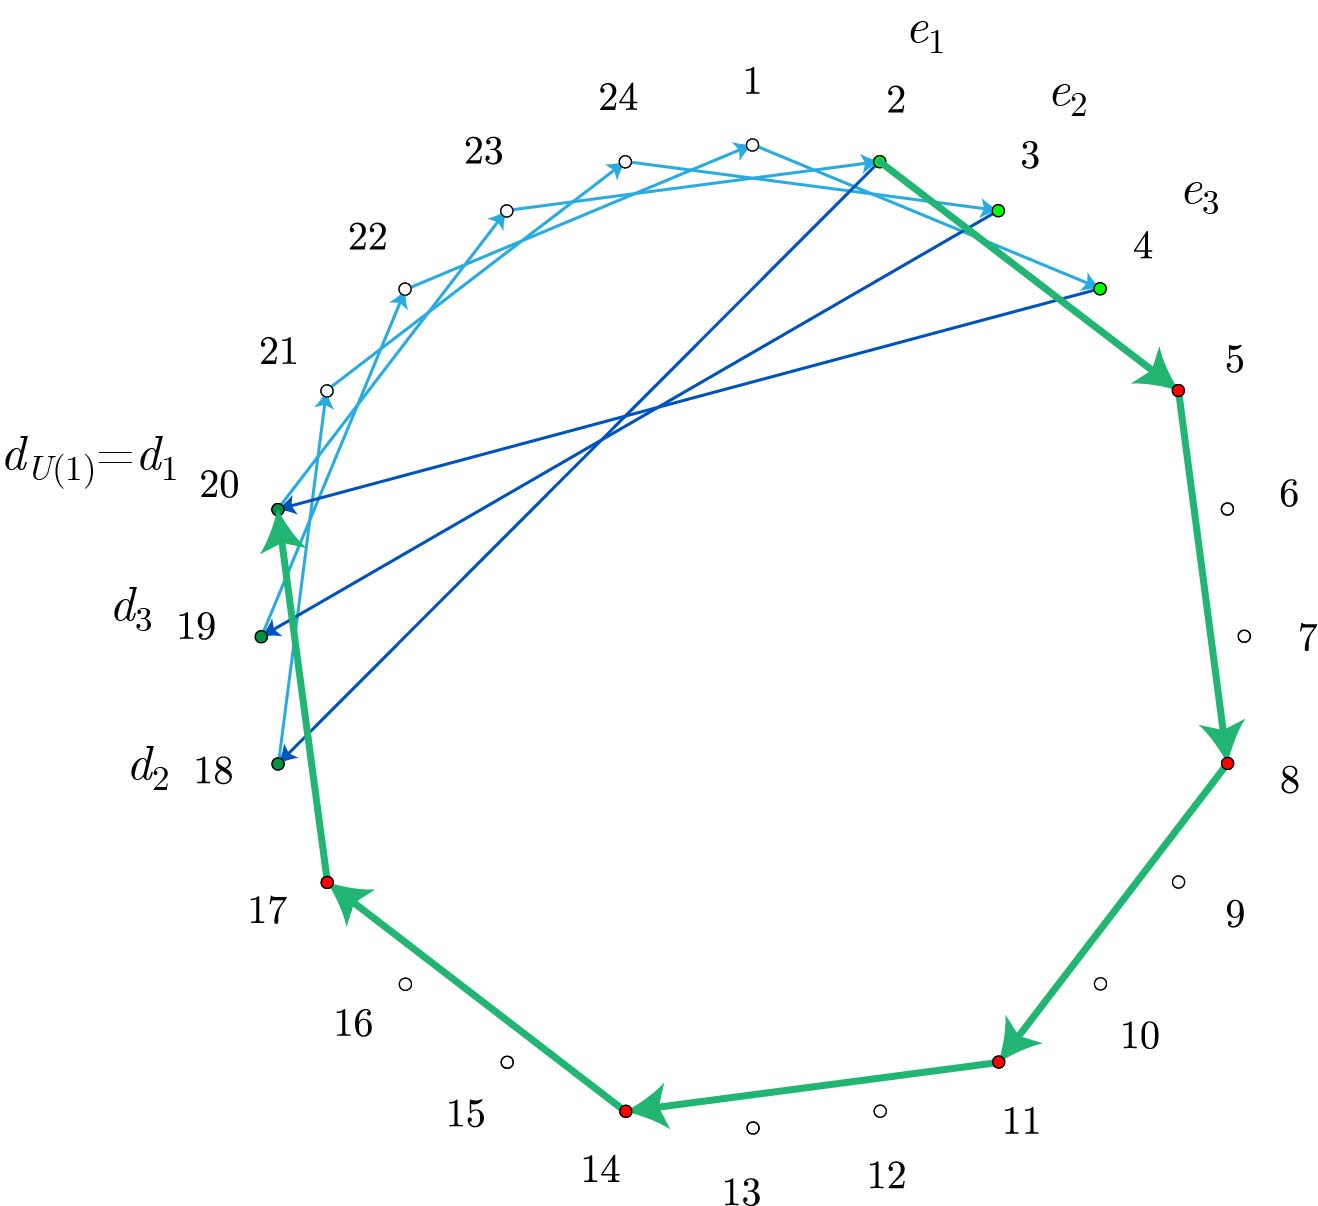
\includegraphics[scale=0.10]{circ_24_U.jpg}
		\caption{The points in red are the points
		in $V_1$. }
	\end{figure}
	\begin{itemize}
		\item Also note that all points in $V_j$
		are fixed by the cycle $C_k$, since any points in 
		$C_k$ are in a sequence of $q_1$-steps starting
		from some $d$ point. 
	\end{itemize}

\end{frame}

%------------------------------------------------

\begin{frame}
\frametitle{Proving Identical Cycle Structure}

	\begin{Def}
		Next we define functions to specify
		the previous element when traversing by
		$q_1$-steps, the next element when
		traversing by $q_1$-steps, and the image of 
		a $q_2$-step from an arbitrary point:
		\bee
			\mathrm{Prev}_{q_1}(x) &= x - q_1 \mod p; \\
			\mathrm{Next}_{q_1}(x) &= x + q_1 \mod p; \\
			\mathrm{Jump}_{q_2}(x) &= x + q_2 \mod p. 
		\eee
	\end{Def}

\end{frame}

%------------------------------------------------

\begin{frame}
\frametitle{Proving Identical Cycle Structure}

	\begin{Def}
		Then we define the $W$-sets
		\bee
			W_j &= \Set{y:(\mathrm{Prev}_{q_1}
			(\mathrm{Jump}_{q_2}(e_j)), y, 
			\mathrm{Next}_{q_1}(e_{j + 1}) 
			\text{ is }q_1\text{-ordered}} \\
			&=
				\Set{y:(\mathrm{Prev}_{q_1}
			(d_{j + 1}), y, 
			\mathrm{Next}_{q_1}(e_{j + 1}) 
			\text{ is }q_1\text{-ordered}}. 
		\eee
	\end{Def}
	\begin{itemize}
		\item Intuitively, these are the points 
		hit in a \textbf{string of $q_1$-steps within
		a cycle} $C_k$, starting with some $d$ point. 
	\end{itemize}

\end{frame}

%------------------------------------------------

\begin{frame}
\frametitle{Proving Identical Cycle Structure}

	\begin{figure}
		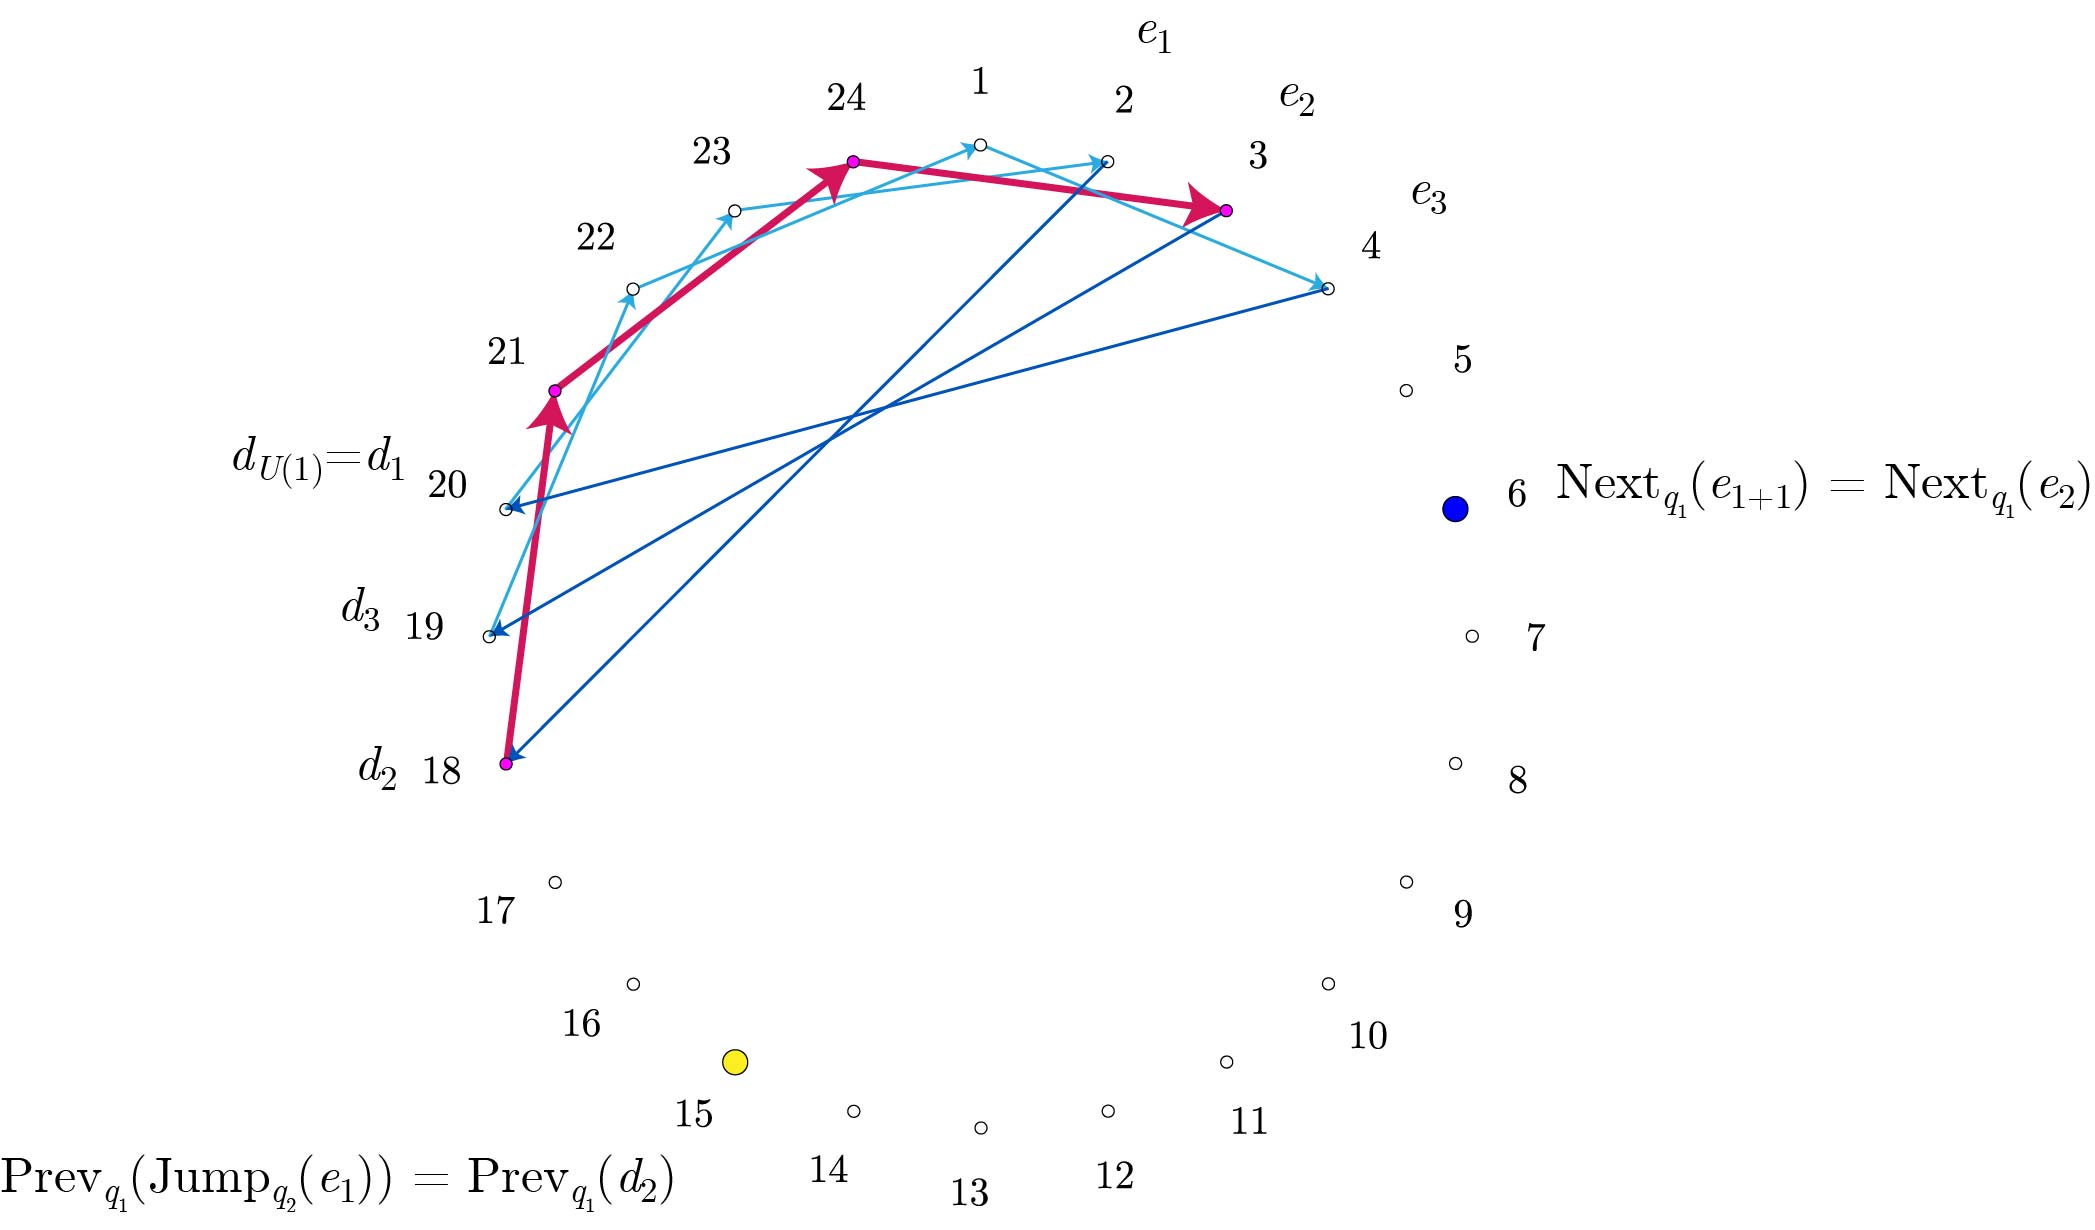
\includegraphics[scale=0.15]{circ_24_W.jpg}
		\caption{The points in $W_1$ are pink. }
	\end{figure}


\end{frame}

%------------------------------------------------

\begin{frame}
\frametitle{Proving Identical Cycle Structure}

	\begin{Prop}
		We claim that for each $x \in V_j$, 
		if $\mathrm{Jump}_{q_2}(x) \in C_k$, 
		then $\mathrm{Jump}_{q_2}(x) \in W_j$, 
		and if $\mathrm{Jump}_{q_2}(x) \notin C_k$, 
		then $\mathrm{Jump}_{q_2}(x) \in V_{j + 1}$. 
	\end{Prop}
	
	\begin{itemize}
		\item We state this without proof for brevity, and 
		instead give visual intuition. 
	\end{itemize}


\end{frame}

%------------------------------------------------

% TODO
% Put in counterexample. 
% Put in illustration for contradiction on slide 64. 
% Make colored dots bigger. 
% Finish Lemma 10. 
% Make diagram for W_j \cup V_{j + 1}.

%------------------------------------------------

\begin{frame}
\frametitle{Proving Identical Cycle Structure}

	\begin{figure}
		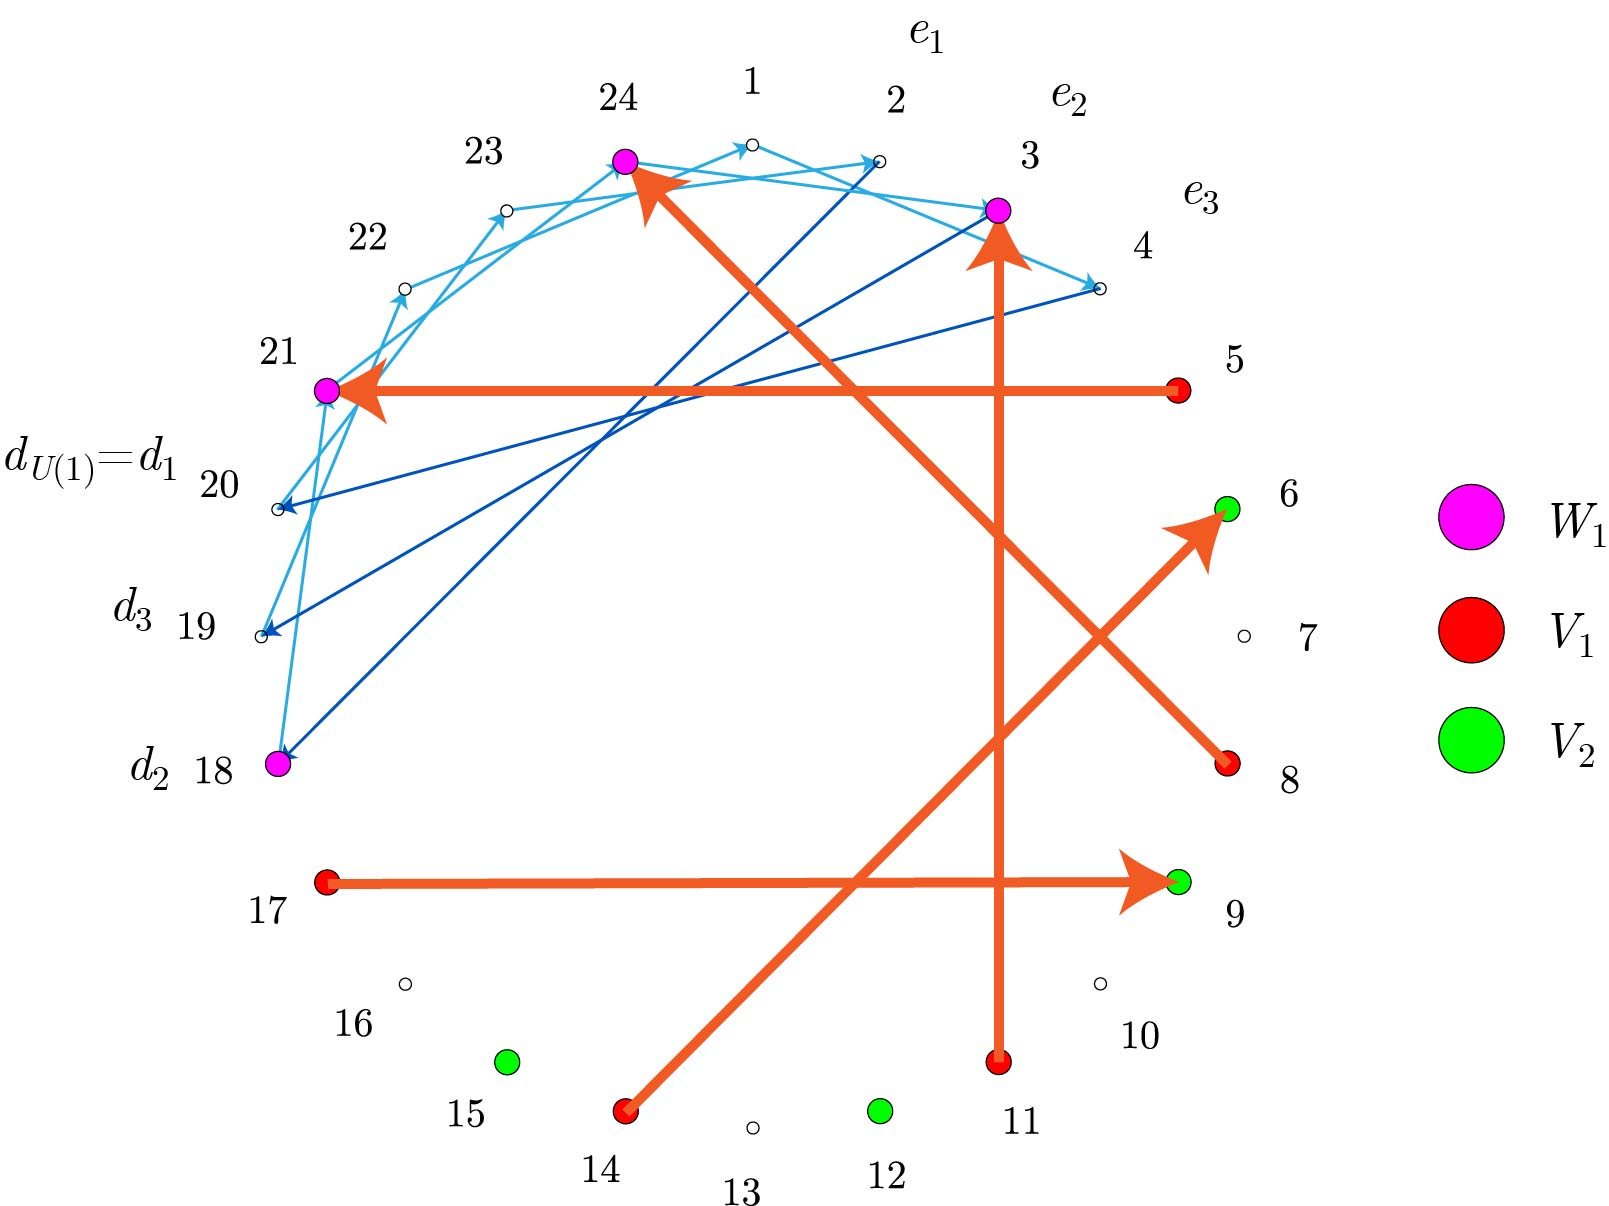
\includegraphics[scale=0.15]{circ_24_VW.jpg}
		\caption{Illustration of $\mathrm{Jump}_{q_1}(x)$
		(orange arrows) for each $x \in V_1$. }
	\end{figure}


\end{frame}

%------------------------------------------------

\begin{comment}

\begin{frame}
\frametitle{Proving Identical Cycle Structure}
	
	\begin{itemize}
		\item Points $x$ in $V_j$ are such that $(e_j,x,d_{U(j)})$
		is $q_1$-ordered. 
		\item The $q_1$-ordered condition is 
		invariant under rotations. 
		\item So 
		\bee
			&(\mathrm{Jump}_{q_2}(e_j),
			\mathrm{Jump}_{q_2}(x),\mathrm{Jump}_{q_2}(d_{U(j)}))\\
			=& 
			(d_{j + 1}, \mathrm{Jump}_{q_2}(x), 
			\mathrm{Jump}_{q_2}(d_{U(j)}))
		\eee
		is also $q_1$-ordered. 
		\item Note $W_j \cup V_{j + 1}$ is the set of 
		all points $y$ such that 
		\bee
			(\mathrm{Prev}_{q_1}(d_{j + 1}), y, 
			d_{U(j + 1)})
		\eee
		is $q_1$-ordered (union of the pink and 
		green points in the example). 
		%\item In this case, $U(2) = 1 + 1 = 2$, but this is not always true, we do not in general havethat $d_{j + 1} = d_{U(j + 1)}$. 
		
		\item We would like to show
		that 
		\bee
			\mathrm{Jump}_{q_1}(x) \in W_j \cup V_{j + 1}
		\eee
		for all $x \in V_j$. 
	\end{itemize}
	% We know that the next $q_2$-step after 
	% d_{U(j)} is e_{U(j)}
	% And Jump(e_{U(j)}) = d_{U(j) + 1}
	% d_{U(j + 1)} = 
	% There is only one d point per equivalence class. 
	% We start at e_{j + 1}, a point somewhere, and 
	% move until we hit the d point in that 
	% equivalence class. 
	
	
	
	%To get to $Jump(e_{U(j)})$, you start at $e_j$ and move a bunchof $q_1$-steps to get to $d_{U(j)}$ and thenyou move a bunch more to get to $e_{U(j)}$, then you take a $q_2$-step. To get to $d_{U(j + 1)}$, you start at $e_j$and take a $q_2$-step to get to $d_{j + 1}$, thenyou take a bunch of $q_1$-steps to get to $e_{j + 1}$, then you take a bunch more to get to$d_{U(j + 1)}$. 
	



\end{frame}



%------------------------------------------------

\begin{frame}
\frametitle{Proving Identical Cycle Structure}
	
	\begin{itemize}
		\item So we want to show that
		\bee
			(d_{j + 1}, \mathrm{Jump}_{q_2}(x), 
			\mathrm{Jump}_{q_2}(d_{U(j)}))
		\eee
		being $q_1$-ordered implies
		\bee
			(\mathrm{Prev}_{q_1}(d_{j + 1}), 
			\mathrm{Jump}_{q_2}(x), 
			d_{U(j + 1)})
		\eee
		is $q_1$-ordered. 
		\item It is sufficient to prove
		\bee
			(\mathrm{Prev}_{q_1}(d_{j + 1}), 
			d_{j + 1}, \mathrm{Jump}_{q_2}(d_{U(j)}),
			d_{U(j + 1)})
		\eee
		is $q_1$-ordered. 
		\item Clearly the first 3 elements are $q_1$-ordered,
		by definition of $\mathrm{Prev}_{q_1}$. 
		
		
	\end{itemize}

\end{frame}

%------------------------------------------------

\begin{frame}
\frametitle{Proving Identical Cycle Structure}
	
	\begin{itemize}
		\item Want to prove that
		\bee
			(\mathrm{Prev}_{q_1}(d_{j + 1}), 
			d_{j + 1}, \mathrm{Jump}_{q_2}(d_{U(j)}),
			d_{U(j + 1)})
		\eee
		is $q_1$-ordered. 
		\item Why are the last 3 elements $q_1$-ordered?
		\item Note
		\bee
			(e_j, d_{U(j)}, e_{U(j)})
		\eee
		is $q_1$-ordered and therefore
		\bee
			&(\mathrm{Jump}_{q_2}(e_j), \mathrm{Jump}_{q_2}(d_{U(j)}), \mathrm{Jump}_{q_2}(e_{U(j)})) \\
			=& (d_{j + 1}, \mathrm{Jump}_{q_2}(d_{U(j)}), 
			d_{U(j) + 1})
		\eee
		is as well. 
		
		
	\end{itemize}

\end{frame}

%------------------------------------------------

\end{comment}









\begin{frame}
\frametitle{Proving Identical Cycle Structure}
	
	\begin{Claim}
		We also claim that each fixed point of $C_k$
		is contained in $V_j$ for some $j$. 
	\end{Claim}
	

\end{frame}

%------------------------------------------------

\begin{frame}
\frametitle{Proving Identical Cycle Structure}
	
	\begin{Claim}
		We also claim that each fixed point of $C_k$
		is contained in $V_j$ for some $j$. 
	\end{Claim}
	\begin{itemize}
		\item We first prove that there is an $e$ point in each
	equivalence class $\mod \gcd(p,q_1)$. 
		\item \textbf{Case 1:}
		If $\gcd(q_1,q_2) = 1$, then we have a $q_2$-step
	($e$ point) in each equivalence class $\mod \gcd(p,q_1)$, 
	since each $q_2$-step takes us to a new equivalence class. 
		\item \textbf{Case 2:} If 
		$\gcd(q_1,q_2) = \psi > 1$, then 
		$\gcd(\psi,p) = \gcd(p,q_1,q_2) = 1$. So we must still
		visit every equivalence class to complete a cycle, and 
		so we have an $e$ point in each. 
	\end{itemize}

\end{frame}

%------------------------------------------------

\begin{frame}
\frametitle{Proving Identical Cycle Structure}
	
	\begin{Claim}
		We also claim that each fixed point of $C_k$
		is contained in $V_j$ for some $j$. 
	\end{Claim}
	\begin{itemize}
		\item So pick a fixed point $x$ of $C_k$. 
		\item Traverse backwards by $q_1$-steps. 
		\item We have just proven you will hit a $q_2$-step
		$e_j$eventually, and before you hit any other point of $C_k$.  
		\item So $x \in V_j$. 
	\end{itemize}

\end{frame}

%------------------------------------------------

\begin{frame}
\frametitle{Proving Identical Cycle Structure}
	
	\begin{rem}
		It is easily proven that the $V_j$ sets do not 
		overlap, so $x$ lies within a unique $V_j$. 
	\end{rem}
	\begin{itemize}
		\item So let $C_l(x) = x$, so $x$ must be a fixed
		point of $C_k$, since the cycles are disjoint. 
		\item We proved that $x$ must be in a unique $V_j$. 
		\item \textbf{Case 1:} $x$ is a $q_1$-step of $C_l$. 
		Then $C_l(x) \in V_j$ as well, since then 
		$C_l(x) = x + q_1$ can only be in $V_j$ or in $C_k$. 
		\item \textbf{Case 2:} $x$ is a $q_2$-step of $C_l$. 
		Then $C_l(x) = x + q_2$ is a fixed point of $C_k$. 
		So $C_l(x) = \mathrm{Jump}_{q_2}(x)$ for $x \in V_j$, 
		so $C_l(x) \in V_{j + 1}$. 
		\item Taking $C_l^t(x)$ and iterating on $t$, 
		i.e. following the orbit of $x$ along the cycle
		$C_l$, we see it must visit each $V_j$ set. 
		\item 
		So we have at least $s_k$ $q_2$-steps in $C_l$.
		
		\item Arguing with roles switched, we have
		at least $s_l$ $q_2$-steps in $C_k$, so $s_l = s_k$. 
	\end{itemize}

\end{frame}

%------------------------------------------------


\begin{frame}
\frametitle{Proving Identical Cycle Structure}
	
	\begin{lem}
		If $T_{p,q_1,q_2}(r,s)$ is nonempty, 
		and $C_i$ is a cycle in $\sigma \in T_{p,q_1,q_2}(r,s)$
		then $p \mid (r_iq_1 + s_iq_2)$. 
		and $p \mid (rq_1 + sq_2)$. 
	\end{lem}
	\begin{itemize}
		\item By the above Lemma stated earlier, we have
		$r_kq_1 + s_kq_2 = \lambda_kp$ and 
		$r_lq_1 + s_kq_2 = \lambda_l p$ 
		for integers $\lambda_k,\lambda_l$, since $s_k = s_l$. 
		\item Then $r_k - r_l = (\lambda_k - \lambda_l)p$. 
		Since $s_k = s_l > 0$, we have
		\bee
			0 &\leq r_k,r_l \leq p - 1\\
			-(p - 1) &\leq r_k - r_l \leq p - 1,
		\eee
		so since $p \mid (r_k - r_l)$, we must have $r_k = r_l$. 
		\item ($q_1,q_2 > 1$, so at most $p/2$ $q_1$-steps. )
		
	\end{itemize}

\end{frame}

%------------------------------------------------

\begin{frame}
\frametitle{Proving Identical Cycle Structure}

	We just proved:
	\begin{lem}
		If $\sigma \in T_{p,q_1,q_2}(r,s)$, 
		and 
		$\gcd(p,q_1,q_2) = 1$, we must have
		$r_1 = r_2 = \cdots = r_k$ and 
		$s_1 = s_2 = \cdots = s_k$. 
	\end{lem}
	
	\begin{theorem}
		If $k$ is the number of cycles in $\sigma$, then
		$k = \gcd(r,s,l)$, $r_i = r/k$, $s_i = s/k$, and
		all permutations in $T_{p,q_1,q_2}(r,s)$ have identical
		cycle structure. 
		So $\mathrm{sgn}(\sigma) = (-1)^{r + s + \gcd(r,s,l)}$. 
	\end{theorem}
	
	\begin{itemize}
		\item We already know $\sum s_i = s$ and $\sum r_i = r$. 
		So by the Lemma we just proved, $s = s_i/k$, and 
		$r = r_i/k$. 
		\item Then
		\bee
			l_i = \fracc{r_iq_1 + s_iq_2}{p} = 
			\fracc{\fracc{rq_1 + sq_2}{p}}{k} = \fracc{l}{k}. 
		\eee
	\end{itemize}

\end{frame}

%------------------------------------------------




%------------------------------------------------

\begin{frame}
\frametitle{Proving Identical Cycle Structure}

	Recall we also stated:
	\begin{lem}
		If $T_{p,q_1,q_2}(r,s)$ is nonempty, 
		then $\gcd(r_i,s_i,l_i) = 1$
		for all $1 \leq i \leq k$, for all
		$\sigma \in T_{p,q_1,q_2}(r,s)$. 
	\end{lem}

	
	\begin{itemize}
		\item So 
		\bee
			k = k\gcd(r_i,s_i,l_i) = \gcd(kr_i,ks_i,kl_i) 
			= \gcd(r,s,l). 
		\eee
		\item So we have determined the number of cycles
		\textbf{from only the parameters} of $T_{p,q_1,q_2}(r,s)$!
		\item Recall the sign of $\sigma$ is defined as 
		$p - c$ where $c$ 
		is the total number of cycles 
		in $\sigma$, including $1$-cycles (fixed points). 
		\item So $c = k + (p - r - s)$. 
		\item So 
		\bee
			\mathrm{sgn}(\sigma) = (-1)^{p - (k + p - r - s)}
			= (-1)^{r + s + \gcd(r,s,l)}. 
		\eee
	\end{itemize}

\end{frame}

%------------------------------------------------

\begin{frame}
\frametitle{Conclusions}

	\begin{itemize}
		\item We have proved the sign of every permutation
		in $T_{p,q_1,q_2}(r,s)$ is the identical. 
		\item So we know the magnitude of the coefficients:
		\bee
			|a_{p,q_1,q_2}(r,s)| = |T_{p,q_1,q_2}(r,s)|. 
		\eee
	\end{itemize}
	Recall we proved:
	\begin{Claim}
		The coefficient of $(-1)^{r + s}x^ry^s$ in $\Theta$
		is the sum of the signs all 
		$\sigma \in T_{p,q_1,q_2}(r,s)$. 
	\end{Claim}
	

\end{frame}

%------------------------------------------------

\begin{frame}
\frametitle{Conclusions}

	Recall we proved:
	\begin{Claim}
		The coefficient of $(-1)^{r + s}x^ry^s$ in $\Theta$
		is the sum of the signs of those permutations in 
		$S_p$ that ``hit'' $r$ of the $-x$'s in the matrix
		and $s$ of the $-y$'s, the remaining values being
		fixed points. 
	\end{Claim}
	
	So we (finally) have
	
	\begin{block}{Formula for Coefficients}
		\bee
			a_{p,q_1,q_2}(r,s) &= (-1)^{r + s}
			|T_{p,q_1,q_2}(r,s)|
			(-1)^{r + s + \gcd(r,s,l)}\\
			&= (-1)^{\gcd(r,s,l)}|T_{p,q_1,q_2}(r,s)|. 
		\eee
	\end{block}
	

\end{frame}

%------------------------------------------------















































%------------------------------------------------

\begin{frame}
\frametitle{References}
% This prints the bibliography on the slide
\nocite{*}
%\bibliographystyle{plain}
\printbibliography
\end{frame}

%----------------------------------------------------------------------------------------

\end{document}
